\begin{figure}[htbp]
    \begin{center}
        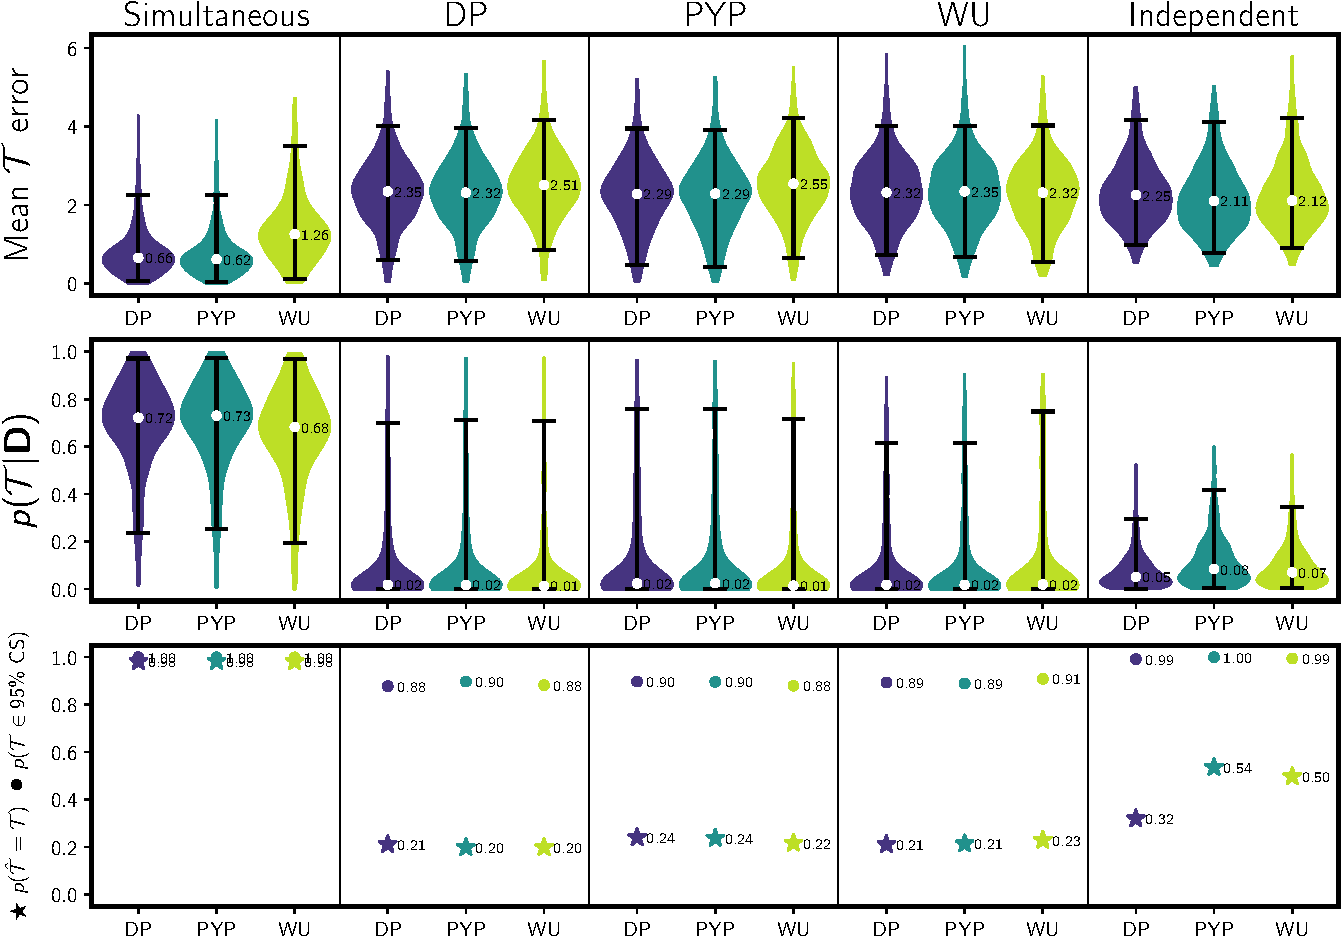
\includegraphics[width=\textwidth,height=\textheight,keepaspectratio]{../images/from-project-repo/var-only-model-performance-violin-cropped.pdf}
        \captionsetup{name=Figure S, labelformat=noSpace, listformat=sFigList}
        \caption{
        Comparing the models' ability to estimate the divergence model
        when using only variable characters from simulated \datasets.
        Each column of plots compares the performance of the Dirichlet process
        (DP), Pitman-Yor process (PYP) and weighted-uniform (\wunif) models when
        analyzing only variable characters from 720 \datasets simulated under
        the (from left-to-right) simultaneous-divergence, DP, PYP, \wunif, and
        independent-divergences model. 
        Mean \etimesets error is the mean partition distance
        of the posterior samples from the true
        divergence model (\etimesets),
        $p(\etimesets \given \alldata)$ is the posterior probability
        of the true divergence model,
        $p(\etimesets \given \alldata)$ is the posterior probability of the
        true divergence model,
        and
        $p(\etimesets \in \textrm{95\% CS})$ is the proportion of simulation
        replicates for which he true \etimesets is included in the 95\%
        posterior credibility set of divergence models.
        The bars overlaying the violin plots show the interval between the
        2.5\% and 97.5\% percentiles, and the white dot is the median.
        We generated the plot using matplotlib Version 3.1.3
        \citep{matplotlib}.
        }
        \label{fig:varonlymodelperformancegrid}
    \end{center}
\end{figure}

\begin{figure}[htbp]
    \begin{center}
        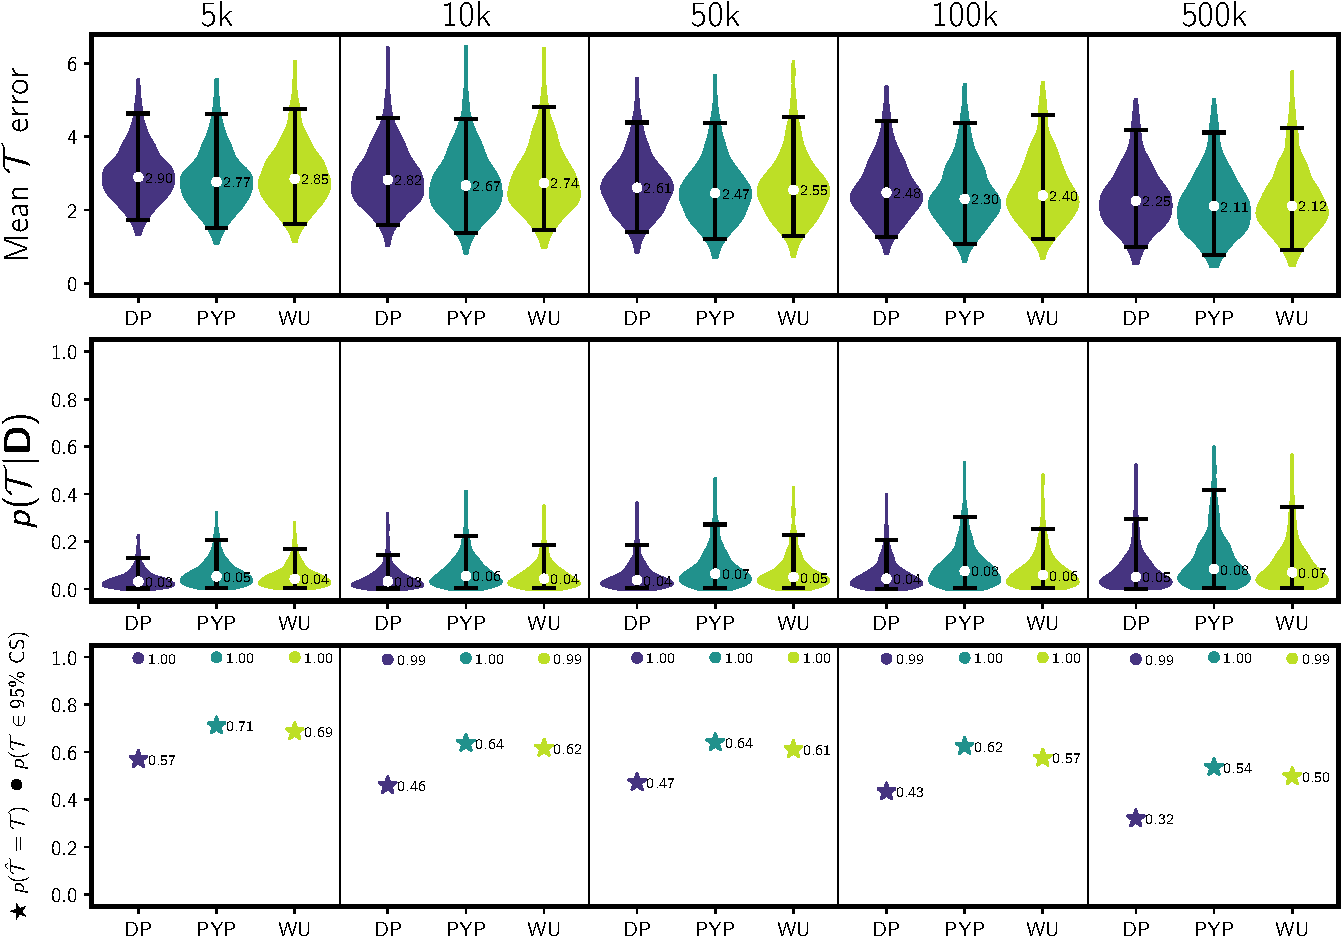
\includegraphics[width=\textwidth,height=\textheight,keepaspectratio]{../images/from-project-repo/var-only-nchars-model-performance-violin-cropped.pdf}
        \captionsetup{name=Figure S, labelformat=noSpace, listformat=sFigList}
        \caption{
        Comparing the models' ability to estimate the independent-divergence
        model when using only variable characters from \datasets of different
        sizes.
        Each column of plots compares the performance of the Dirichlet process
        (DP), Pitman-Yor process (PYP) and weighted-uniform (\wunif) models when
        analyzing only variable characters from 720 \datasets with 5,000 to
        500,000 characters simulated under the independent-divergences model.
        Mean \etimesets error is the mean partition distance
        of the posterior samples from the true
        divergence model (\etimesets),
        $p(\etimesets \given \alldata)$ is the posterior probability
        of the true divergence model,
        $p(\etimesets \given \alldata)$ is the posterior probability of the
        true divergence model,
        and
        $p(\etimesets \in \textrm{95\% CS})$ is the proportion of simulation
        replicates for which he true \etimesets is included in the 95\%
        posterior credibility set of divergence models.
        The bars overlaying the violin plots show the interval between the
        2.5\% and 97.5\% percentiles, and the white dot is the median.
        We generated the plot using matplotlib Version 3.1.3
        \citep{matplotlib}.
        }
        \label{fig:varonlymodelperformancebysize}
    \end{center}
\end{figure}

\begin{figure}[htbp]
    \begin{center}
        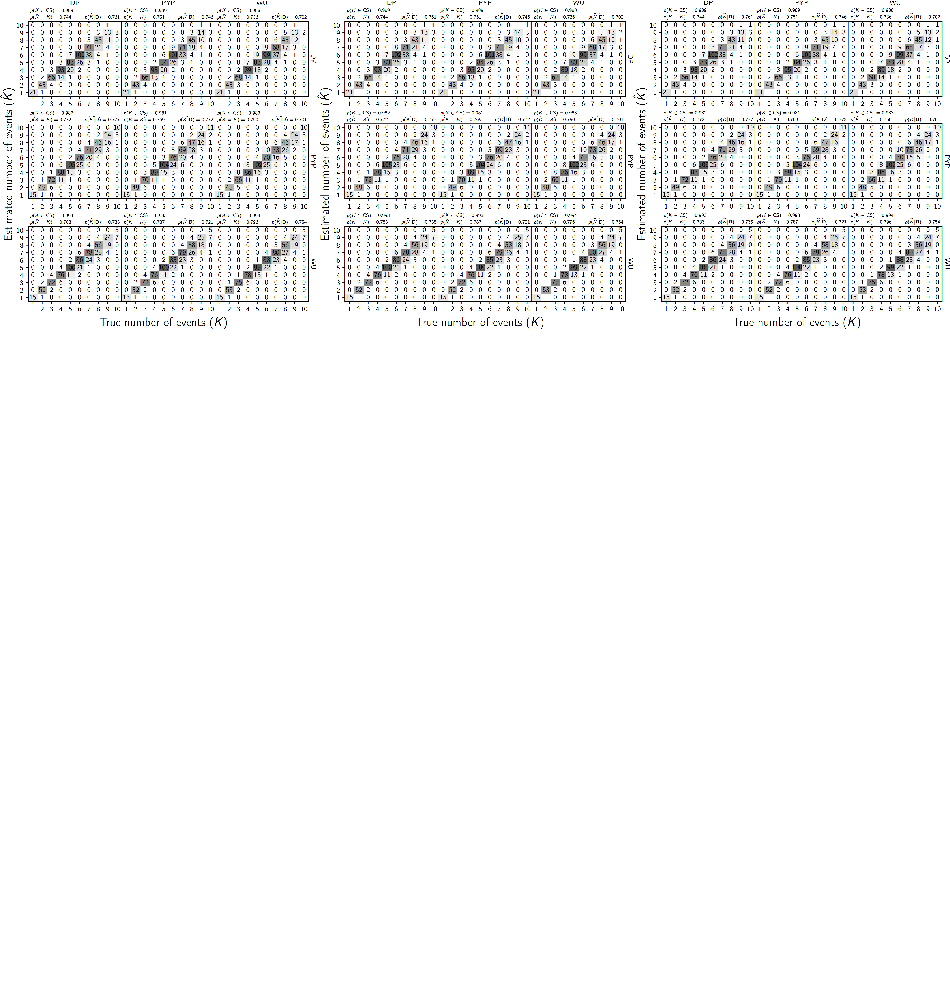
\includegraphics[width=\textwidth,height=\textheight,keepaspectratio]{../images/from-project-repo/infer-columns-by-data-rows-nevents-cropped-rasterized.pdf}
        \captionsetup{name=Figure S, labelformat=noSpace, listformat=sFigList}
        \caption{
        The models perform similarly in estimating the number of divergence
        events.
        Each plot shows the results for 720 \datasets
        simulated under the
        DP (top row),
        PYP (middle row),
        or
        \wunif (bottom row)
        and analyses using the
        DP (left column),
        PYP (middle column),
        or
        \wunif (right column).
        The number of \datasets that fall within each possible cell of true
        versus estimated numbers of events is shown, and cells with more
        \datasets are shaded darker.
        % The estimates are based on the number of events with the maximum
        % \textit{a posteriori} (MAP) probability.
        Above each plot is
        the proportion of \datasets for which the number of events with the largest
        posterior probability matched the true number of events---$p(\hat{\nevents}
        = \nevents)$,
        the median posterior probability of the correct number of events across all
        \datasets---$\widetilde{p(\nevents|\alldata)}$, and
        the proportion of \datasets for which the true number of events was
        included in the 95\% credible set---$p(\nevents \in
        \textrm{CS})$.
        We generated the plot using matplotlib Version 3.1.3
        \citep{matplotlib}.
        }
        \label{fig:neventsgrid}
    \end{center}
\end{figure}

\begin{figure}[htbp]
    \begin{center}
        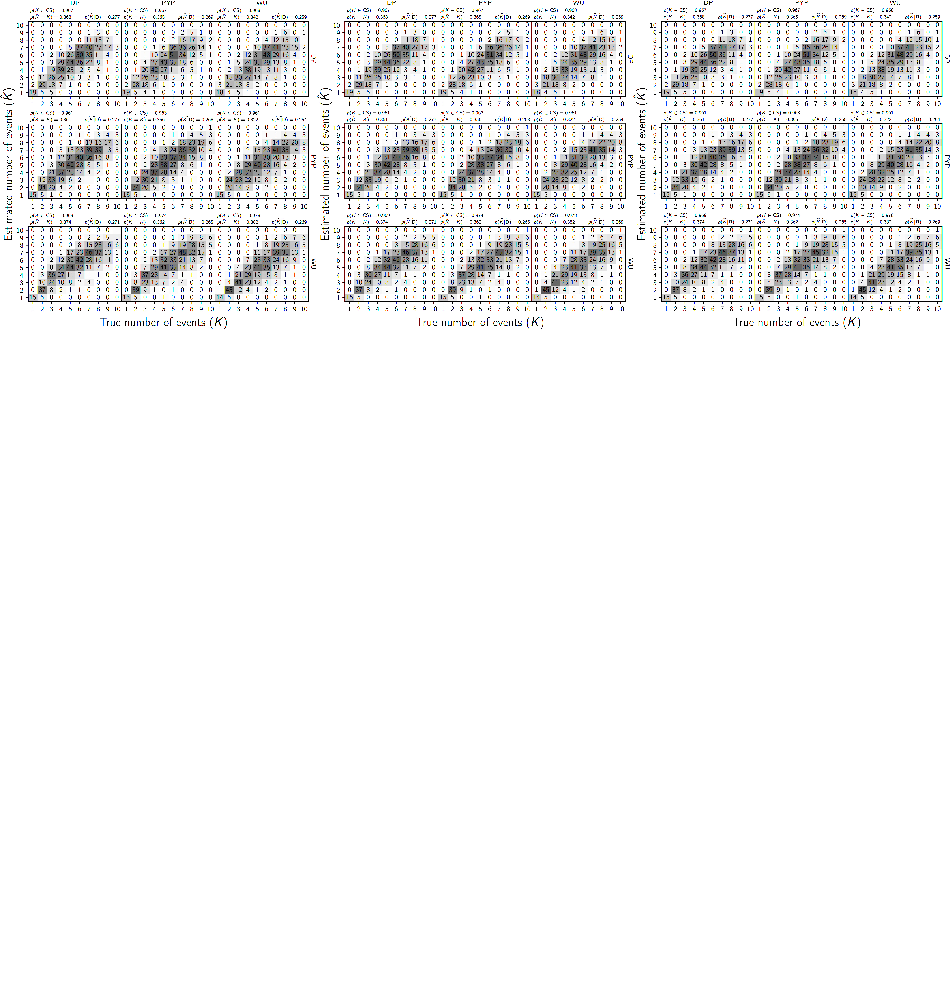
\includegraphics[width=\textwidth,height=\textheight,keepaspectratio]{../images/from-project-repo/var-only-infer-columns-by-data-rows-nevents-cropped-rasterized.pdf}
        \captionsetup{name=Figure S, labelformat=noSpace, listformat=sFigList}
        \caption{
        The models perform similarly in estimating the number of divergence
        events when using only variable characters from the simulated
        \datasets.
        Each plot shows the results from using only variable characters from
        720 \datasets simulated under the
        DP (top row),
        PYP (middle row),
        or
        \wunif (bottom row)
        and analyses using the
        DP (left column),
        PYP (middle column),
        or
        \wunif (right column).
        The number of \datasets that fall within each possible cell of true
        versus estimated numbers of events is shown, and cells with more
        \datasets are shaded darker.
        % The estimates are based on the number of events with the maximum
        % \textit{a posteriori} (MAP) probability.
        Above each plot is
        the proportion of \datasets for which the number of events with the largest
        posterior probability matched the true number of events---$p(\hat{\nevents}
        = \nevents)$,
        the median posterior probability of the correct number of events across all
        \datasets---$\widetilde{p(\nevents|\alldata)}$, and
        the proportion of \datasets for which the true number of events was
        included in the 95\% credible set---$p(\nevents \in
        \textrm{CS})$.
        We generated the plot using matplotlib Version 3.1.3
        \citep{matplotlib}.
        }
        \label{fig:varonlyneventsgrid}
    \end{center}
\end{figure}

\begin{figure}[htbp]
    \begin{center}
        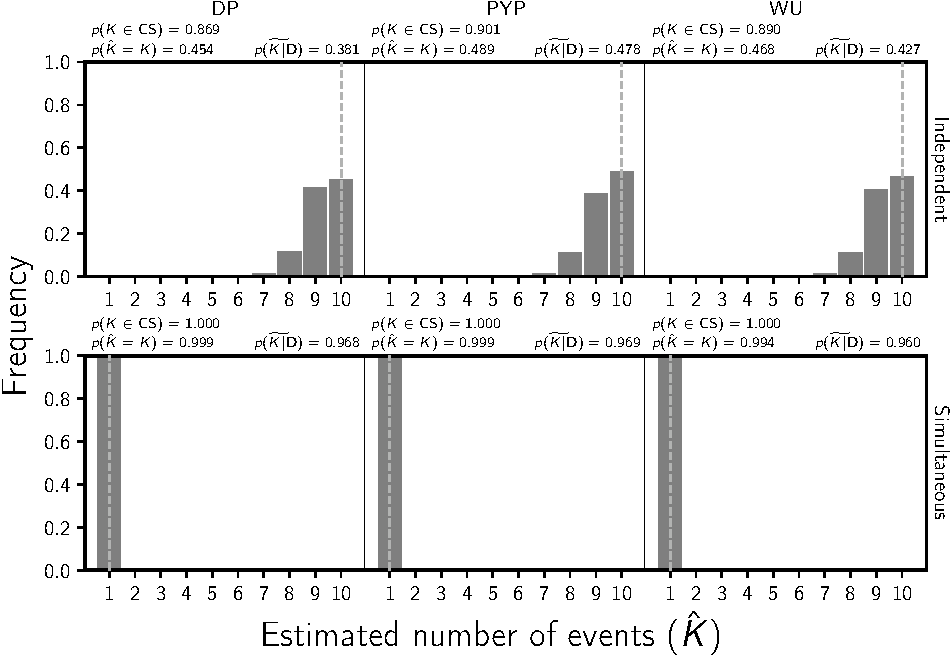
\includegraphics[width=\textwidth,height=\textheight,keepaspectratio]{../images/from-project-repo/infer-columns-by-fixed-rows-nevents-cropped.pdf}
        \captionsetup{name=Figure S, labelformat=noSpace, listformat=sFigList}
        \caption{
        The PYP (middle column) model performs better than the DP (left column)
        and \wunif (right column) models when analyzing simulated \datasets for
        which all 10 population pairs diverged independently (top row).
        All three models almost always correctly infer a single shared
        divergence event with high confidence when analyzing simulated
        \datasets for which that is true (bottom row).
        Each plot shows the results for 720 \datasets.
        Above each plot is
        the proportion of \datasets for which the number of events with the largest
        posterior probability matched the true number of events---$p(\hat{\nevents}
        = \nevents)$,
        the median posterior probability of the correct number of events across all
        \datasets---$\widetilde{p(\nevents|\alldata)}$, and
        the proportion of \datasets for which the true number of events was
        included in the 95\% credible set---$p(\nevents \in
        \textrm{CS})$.
        We generated the plot using matplotlib Version 3.1.3
        \citep{matplotlib}.
        }
        \label{fig:neventsfixedcomparison}
    \end{center}
\end{figure}

\begin{figure}[htbp]
    \begin{center}
        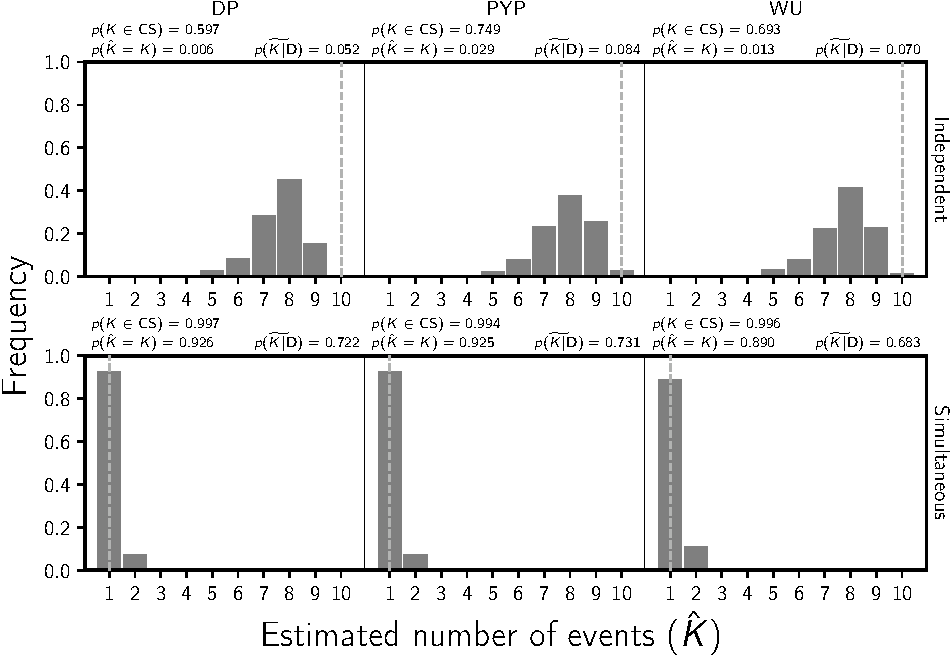
\includegraphics[width=\textwidth,height=\textheight,keepaspectratio]{../images/from-project-repo/var-only-infer-columns-by-fixed-rows-nevents-cropped.pdf}
        \captionsetup{name=Figure S, labelformat=noSpace, listformat=sFigList}
        \caption{
        The PYP (middle column) model performs better than the DP (left column)
        and \wunif (right column) models when analyzing only variable characters
        from simulated \datasets for which all 10 population pairs diverged
        independently (top row).
        All three models perform well at correctly infer a single shared
        divergence event when analyzing simulated \datasets for which that is
        true (bottom row), although the \wunif model does not perform quite as
        well as the DP and PYP models.
        Each plot shows the results from using only variable characters from
        720 \datasets.
        Above each plot is
        the proportion of \datasets for which the number of events with the largest
        posterior probability matched the true number of events---$p(\hat{\nevents}
        = \nevents)$,
        the median posterior probability of the correct number of events across all
        \datasets---$\widetilde{p(\nevents|\alldata)}$, and
        the proportion of \datasets for which the true number of events was
        included in the 95\% credible set---$p(\nevents \in
        \textrm{CS})$.
        We generated the plot using matplotlib Version 3.1.3
        \citep{matplotlib}.
        }
        \label{fig:varonlyneventsfixedcomparison}
    \end{center}
\end{figure}

\begin{figure}[htbp]
    \begin{center}
        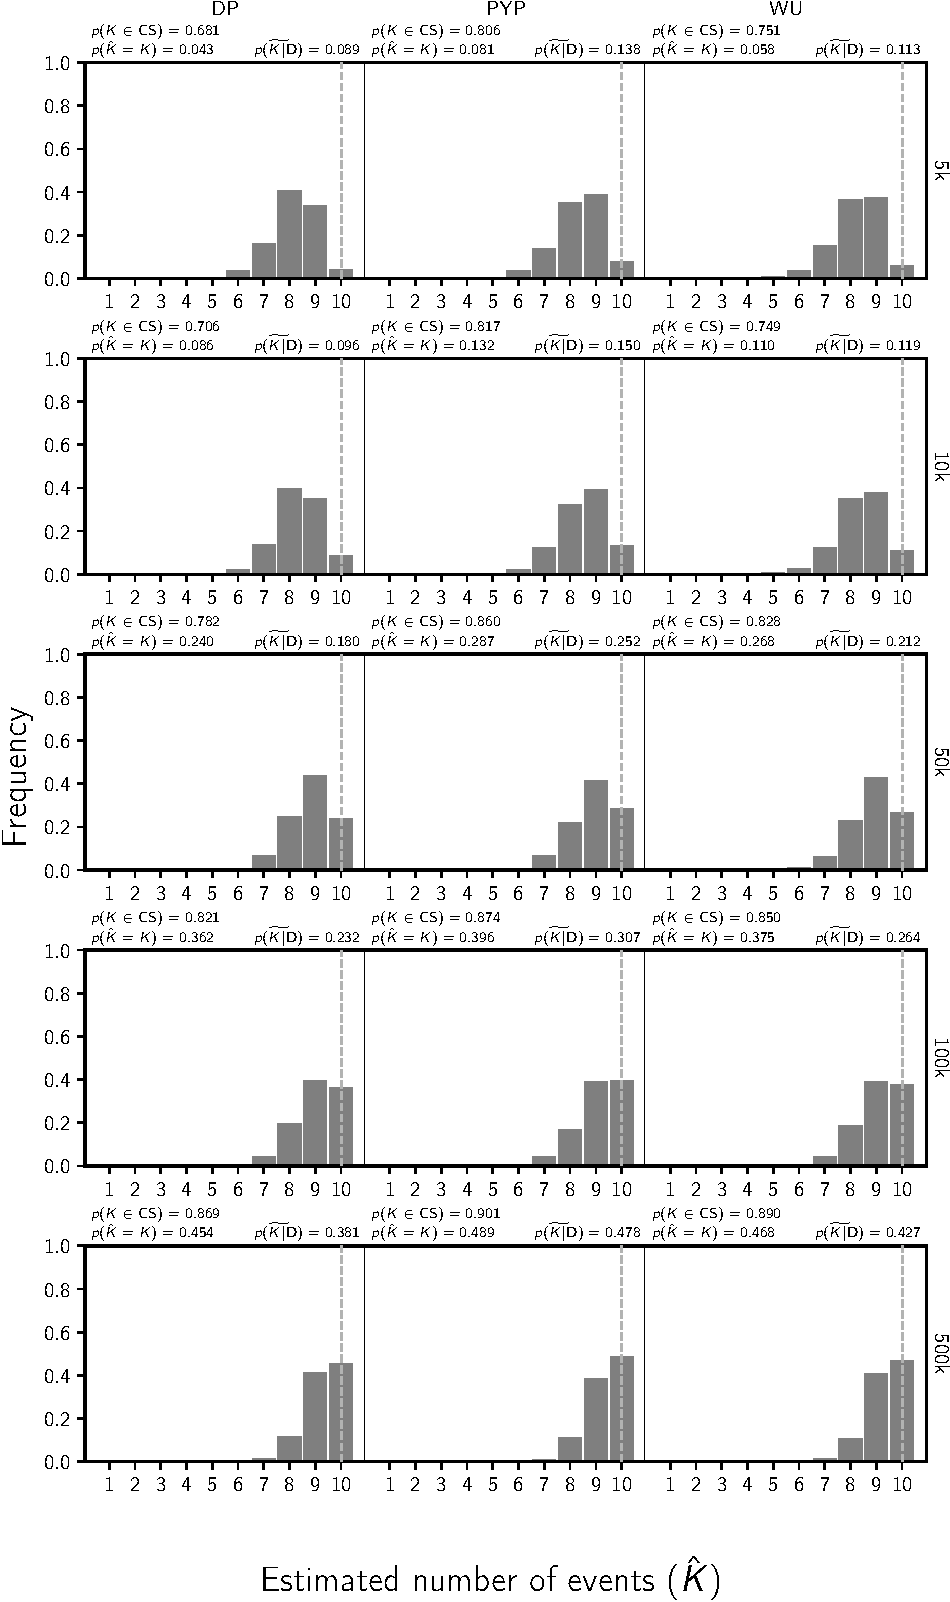
\includegraphics[width=\textwidth,height=0.9\textheight,keepaspectratio]{../images/from-project-repo/nchars-nevents-cropped.pdf}
        \captionsetup{name=Figure S, labelformat=noSpace, listformat=sFigList}
        \caption{\scriptsize
        The PYP (middle column) model performs better than the DP (left column)
        and \wunif (right column) models when analyzing \datasets of different
        sizes simulated under the independent-divergences model.
        Each plot shows the results for 720 \datasets with 5,000 to
        500,000 characters simulated under the independent-divergences model.
        Above each plot is
        the proportion of \datasets for which the number of events with the largest
        posterior probability matched the true number of events---$p(\hat{\nevents}
        = \nevents)$,
        the median posterior probability of the correct number of events across all
        \datasets---$\widetilde{p(\nevents|\alldata)}$, and
        the proportion of \datasets for which the true number of events was
        included in the 95\% credible set---$p(\nevents \in
        \textrm{CS})$.
        We generated the plot using matplotlib Version 3.1.3
        \citep{matplotlib}.
        }
        \label{fig:neventsgridbysize}
    \end{center}
\end{figure}

\begin{figure}[htbp]
    \begin{center}
        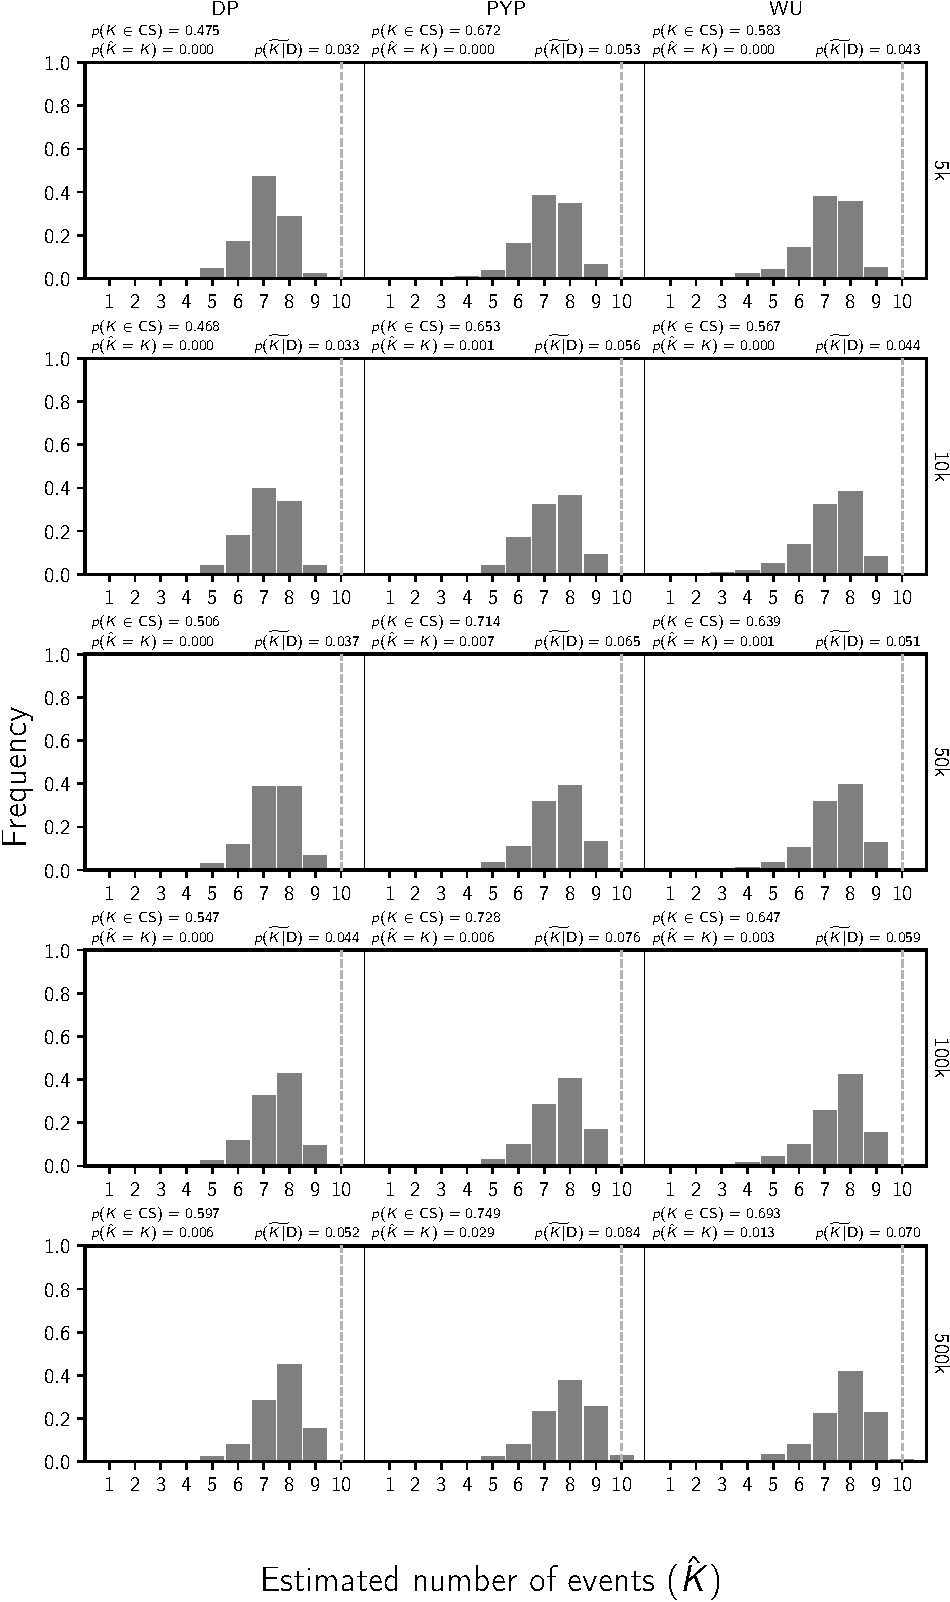
\includegraphics[width=\textwidth,height=0.9\textheight,keepaspectratio]{../images/from-project-repo/var-only-nchars-nevents-cropped.pdf}
        \captionsetup{name=Figure S, labelformat=noSpace, listformat=sFigList}
        \caption{\scriptsize
        The PYP (middle column) model performs better than the DP (left column)
        and \wunif (right column) models when analyzing only variable characters
        from \datasets of different sizes simulated under the
        independent-divergences model.
        Each plot shows the results from 720 \datasets when analyzing only the
        variable characters out of 5,000 to 500,000 characters simulated under
        the independent-divergences model.
        Above each plot is
        the proportion of \datasets for which the number of events with the largest
        posterior probability matched the true number of events---$p(\hat{\nevents}
        = \nevents)$,
        the median posterior probability of the correct number of events across all
        \datasets---$\widetilde{p(\nevents|\alldata)}$, and
        the proportion of \datasets for which the true number of events was
        included in the 95\% credible set---$p(\nevents \in
        \textrm{CS})$.
        We generated the plot using matplotlib Version 3.1.3
        \citep{matplotlib}.
        }
        \label{fig:varonlyneventsgridbysize}
    \end{center}
\end{figure}

\begin{figure}[htbp]
    \begin{center}
        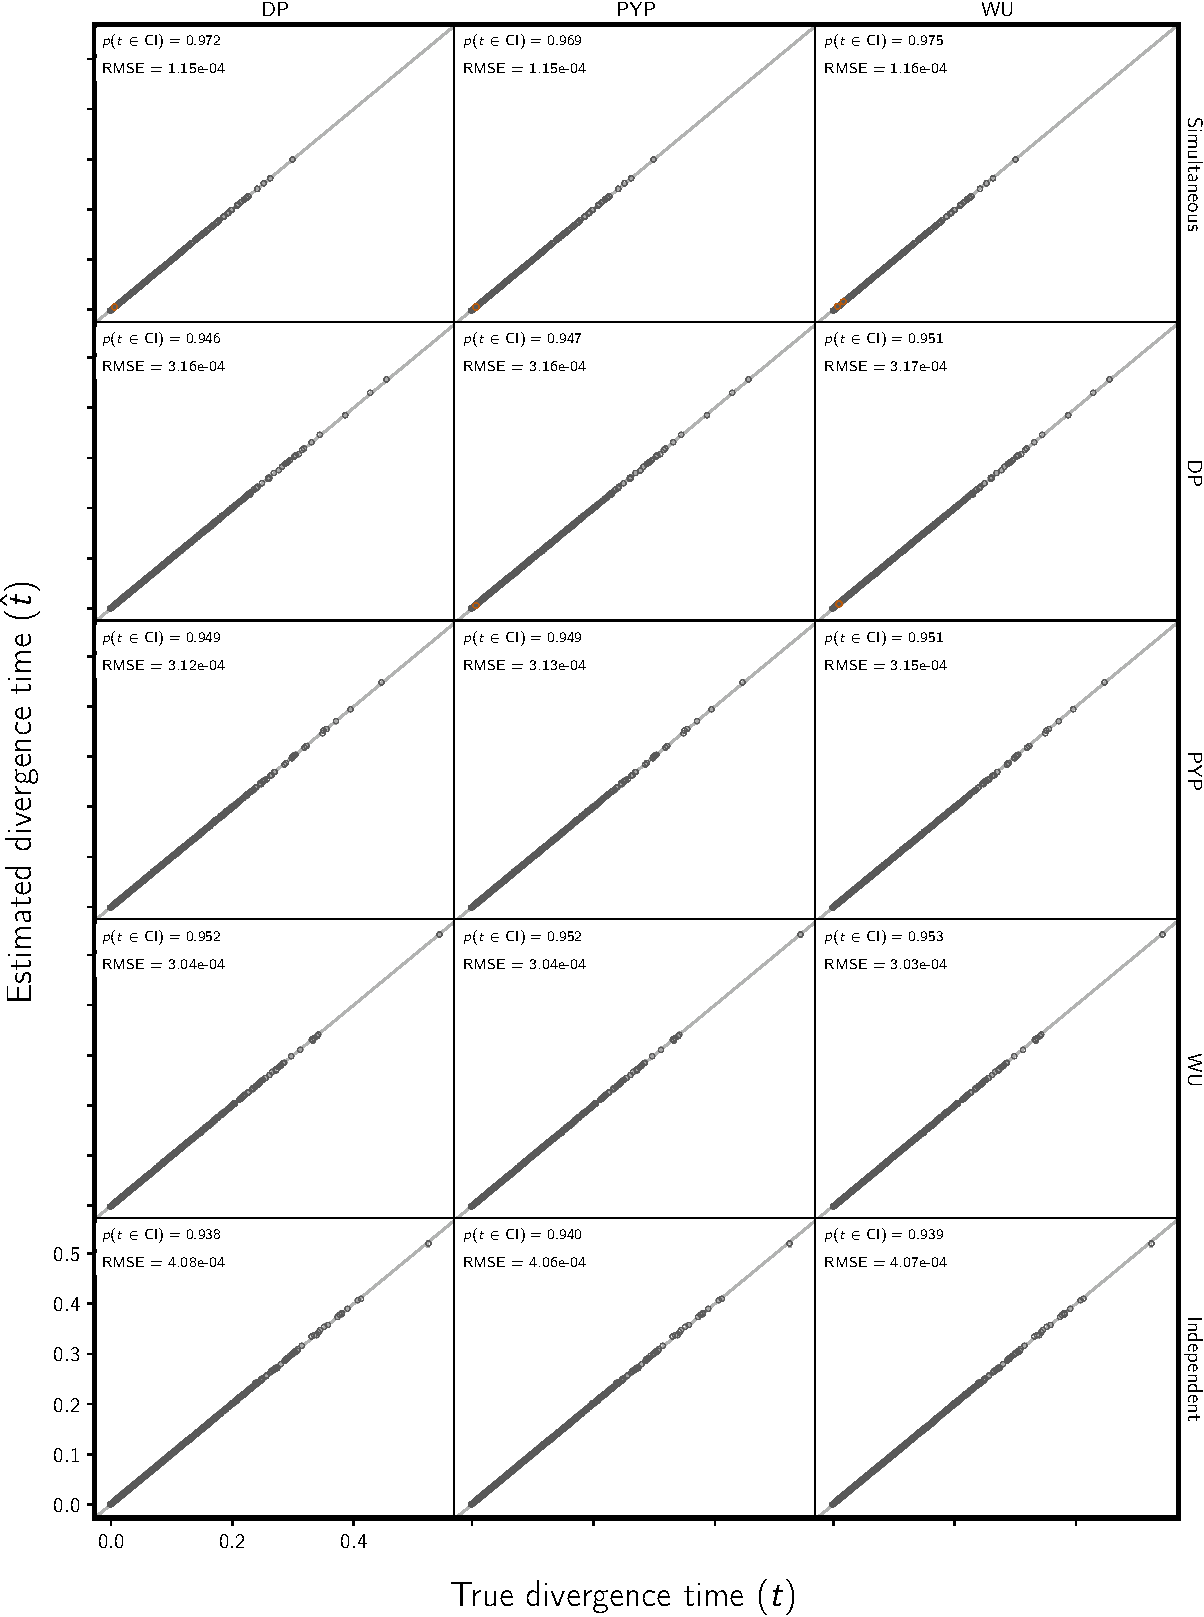
\includegraphics[width=\textwidth,height=0.9\textheight,keepaspectratio]{../images/from-project-repo/infer-columns-by-data-rows-div-time-scatter-cropped.pdf}
        \captionsetup{name=Figure S, labelformat=noSpace, listformat=sFigList}
        \caption{\footnotesize
        The DP (left column),
        PYP (middle column),
        and
        \wunif
        perform similarly well at estimating the divergence times from
        \datasets simulated under five different models (see row labels) with
        500,000 characters from 10 pairs of populations.
        At the top of each plot is the root-mean-square error (RMSE)
        and
        the proportion of \datasets for which the true divergence time was
        included in the 95\% credible interval---$p(\comparisonetime \in
        \textrm{CS})$.
        Estimates for which the potential-scale reduction factor was greater
        than 1.2 \citep{Brooks1998} are highlighted in orange.
        We generated the plot using matplotlib Version 3.1.3
        \citep{matplotlib}.
        }
        \label{fig:divtimegrid}
    \end{center}
\end{figure}

\begin{figure}[htbp]
    \begin{center}
        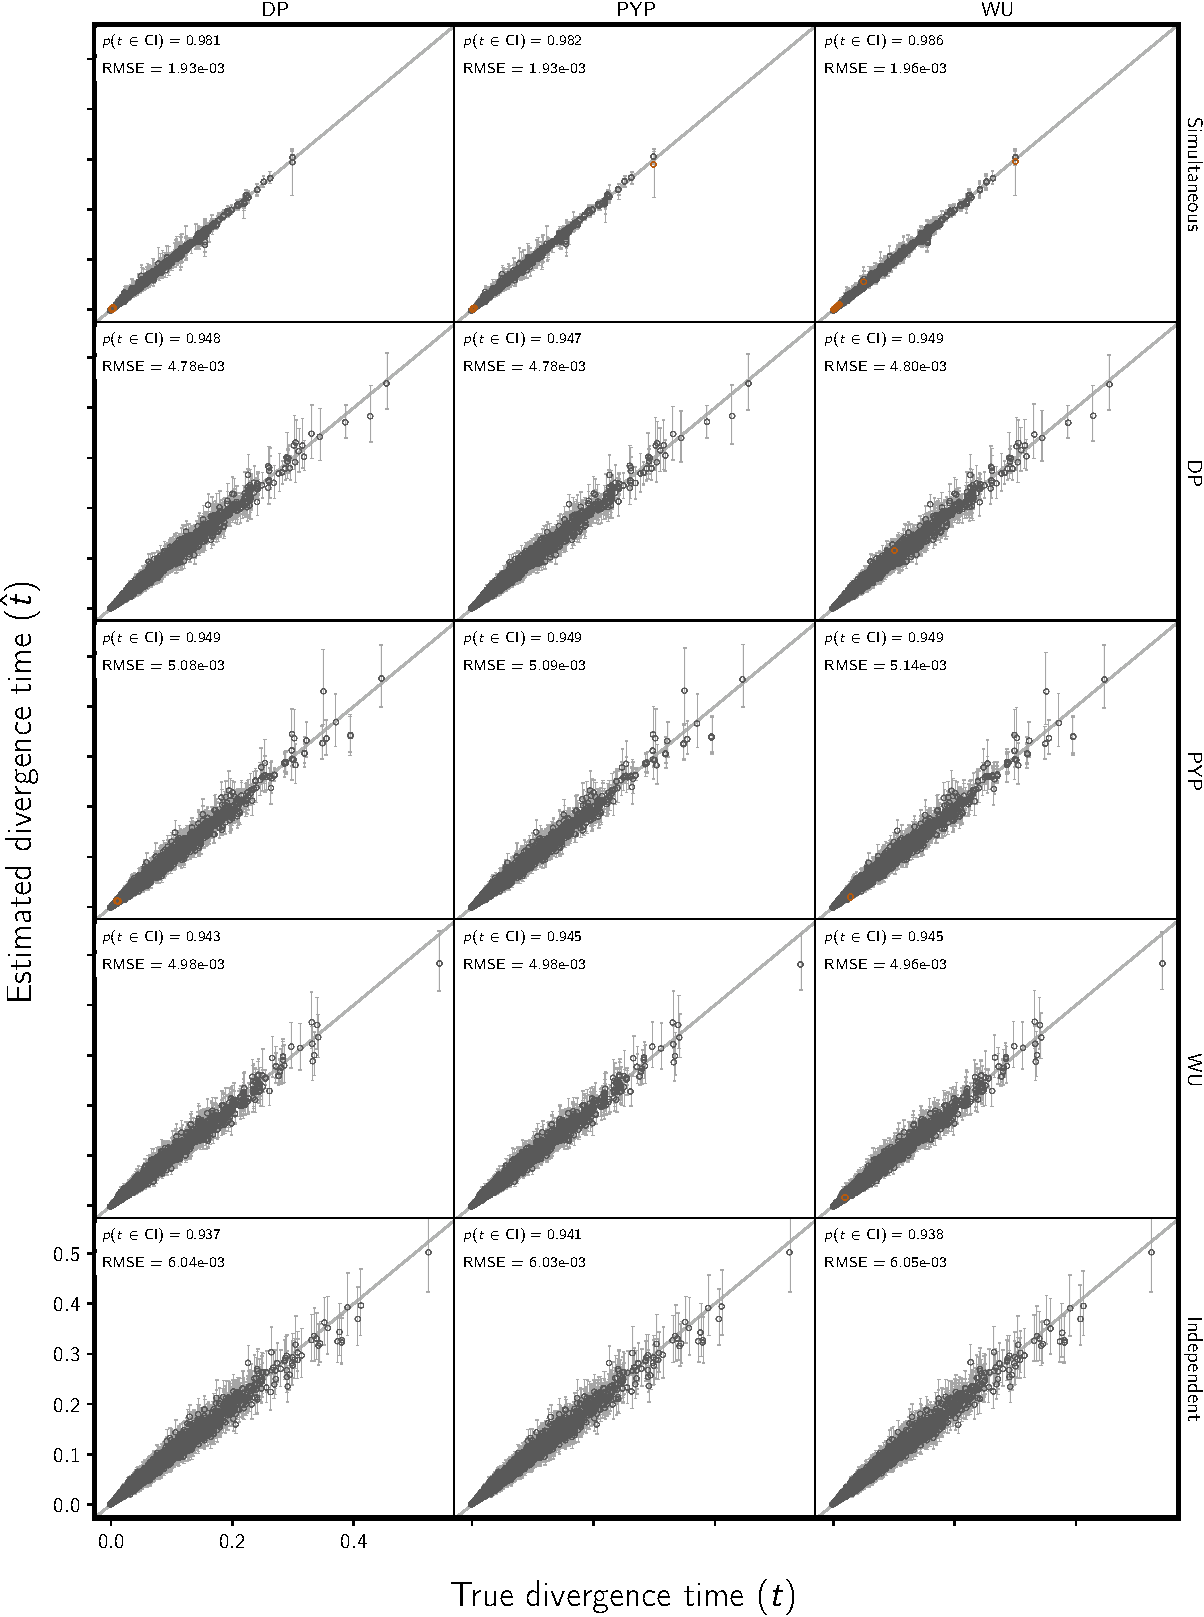
\includegraphics[width=\textwidth,height=0.9\textheight,keepaspectratio]{../images/from-project-repo/var-only-infer-columns-by-data-rows-div-time-scatter-cropped.pdf}
        \captionsetup{name=Figure S, labelformat=noSpace, listformat=sFigList}
        \caption{\footnotesize
        The DP (left column),
        PYP (middle column),
        and
        \wunif
        perform similarly at estimating the divergence times from only the
        variable characters from \datasets simulated under five different
        models (see row labels) with 10 pairs of populations.
        At the top of each plot is the root-mean-square error (RMSE)
        and
        the proportion of \datasets for which the true divergence time was
        included in the 95\% credible interval---$p(\comparisonetime \in
        \textrm{CS})$.
        Estimates for which the potential-scale reduction factor was greater
        than 1.2 \citep{Brooks1998} are highlighted in orange.
        We generated the plot using matplotlib Version 3.1.3
        \citep{matplotlib}.
        }
        \label{fig:varonlydivtimegrid}
    \end{center}
\end{figure}

\begin{figure}[htbp]
    \begin{center}
        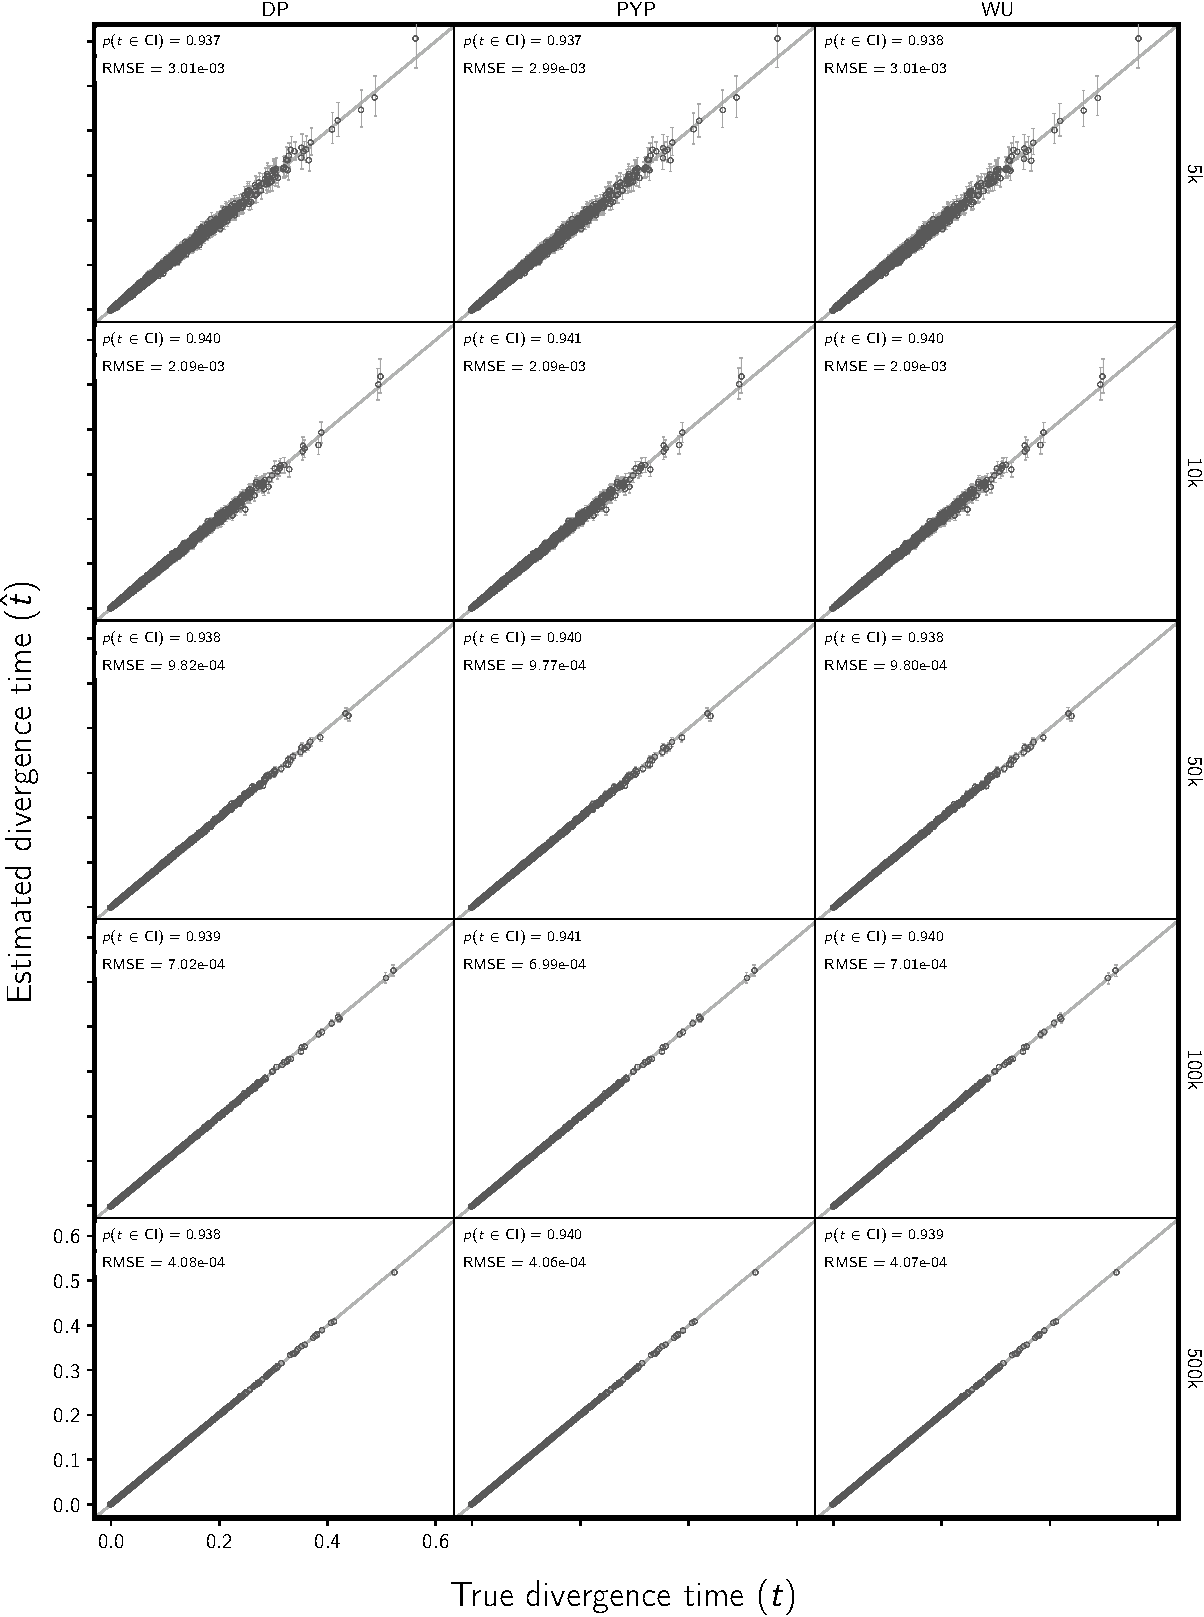
\includegraphics[width=\textwidth,height=0.9\textheight,keepaspectratio]{../images/from-project-repo/nchars-div-time-scatter-cropped.pdf}
        \captionsetup{name=Figure S, labelformat=noSpace, listformat=sFigList}
        \caption{\footnotesize
        The DP (left column),
        PYP (middle column),
        and
        \wunif
        perform similarly well at estimating the divergence times from
        \datasets of varying size (see row labels) simulated with
        10 pairs of populations diverging independently.
        At the top of each plot is the root-mean-square error (RMSE)
        and
        the proportion of \datasets for which the true divergence time was
        included in the 95\% credible interval---$p(\comparisonetime \in
        \textrm{CS})$.
        Estimates for which the potential-scale reduction factor was greater
        than 1.2 \citep{Brooks1998} are highlighted in orange.
        We generated the plot using matplotlib Version 3.1.3
        \citep{matplotlib}.
        }
        \label{fig:divtimegridbysize}
    \end{center}
\end{figure}

\begin{figure}[htbp]
    \begin{center}
        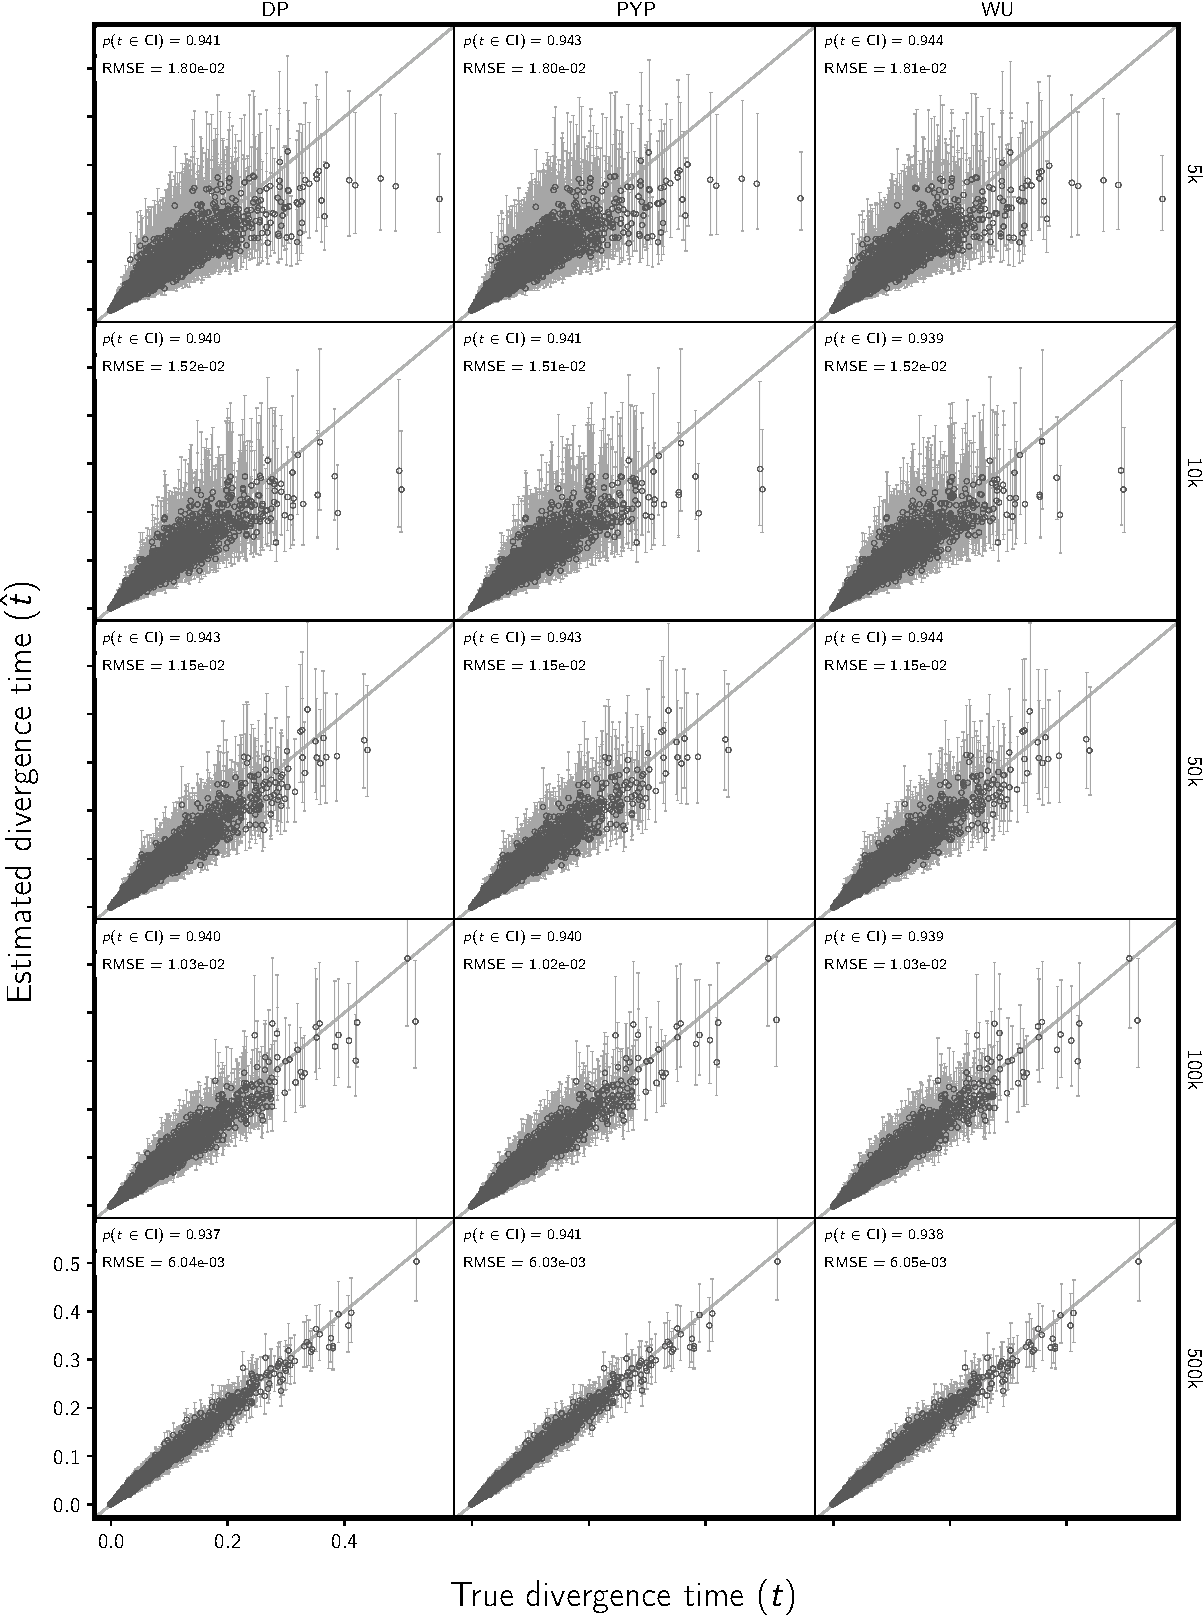
\includegraphics[width=\textwidth,height=0.9\textheight,keepaspectratio]{../images/from-project-repo/var-only-nchars-div-time-scatter-cropped.pdf}
        \captionsetup{name=Figure S, labelformat=noSpace, listformat=sFigList}
        \caption{\footnotesize
        The DP (left column),
        PYP (middle column),
        and
        \wunif
        perform similarly at estimating the divergence times from only the
        variable characters from \datasets of varying size (see row labels)
        simulated with 10 pairs of populations diverging independently.
        At the top of each plot is the root-mean-square error (RMSE)
        and
        the proportion of \datasets for which the true divergence time was
        included in the 95\% credible interval---$p(\comparisonetime \in
        \textrm{CS})$.
        Estimates for which the potential-scale reduction factor was greater
        than 1.2 \citep{Brooks1998} are highlighted in orange.
        We generated the plot using matplotlib Version 3.1.3
        \citep{matplotlib}.
        }
        \label{fig:varonlydivtimegridbysize}
    \end{center}
\end{figure}



% Ancestral population size

\begin{figure}[htbp]
    \begin{center}
        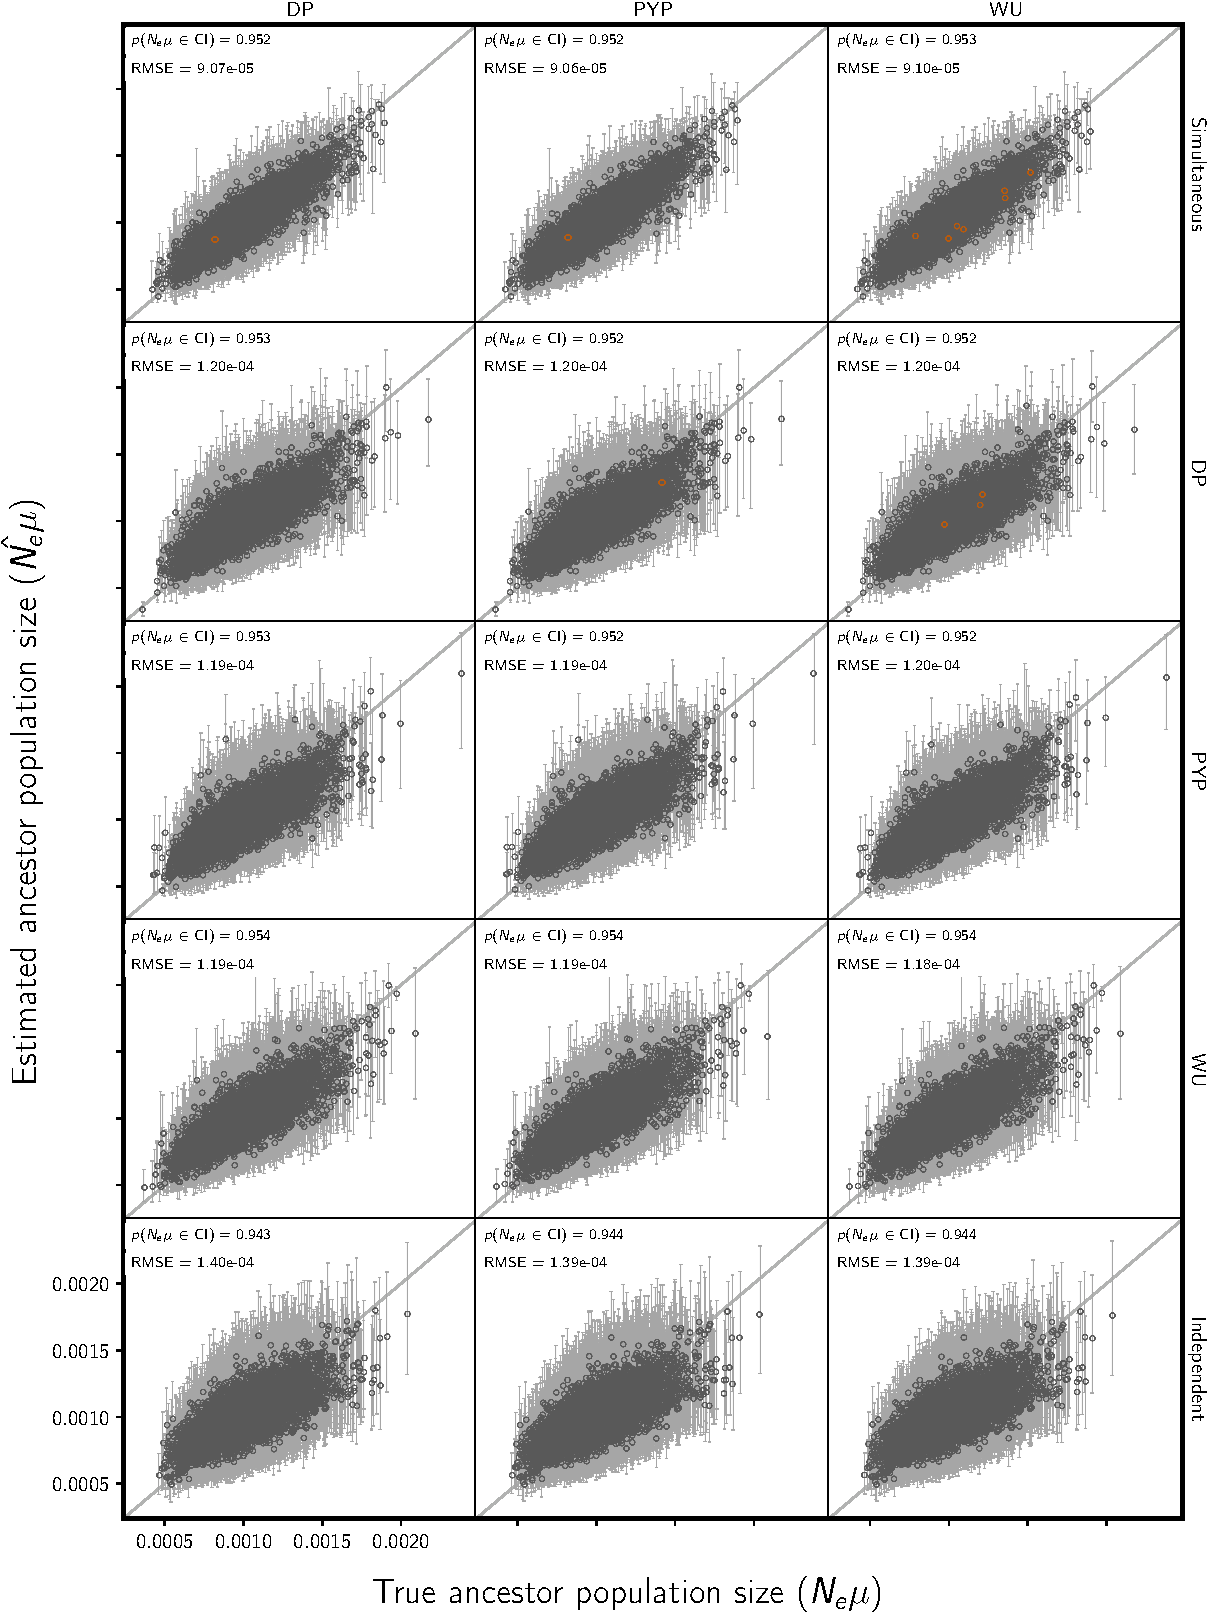
\includegraphics[width=\textwidth,height=0.9\textheight,keepaspectratio]{../images/from-project-repo/infer-columns-by-data-rows-ancestor-size-scatter-cropped.pdf}
        \captionsetup{name=Figure S, labelformat=noSpace, listformat=sFigList}
        \caption{\footnotesize
        The DP (left column),
        PYP (middle column),
        and
        \wunif
        perform similarly at estimating the effective size of the
        ancestral populations from \datasets simulated under five different
        models (see row labels) with 500,000 characters from 10 pairs of
        populations.
        At the top of each plot is the root-mean-square error (RMSE)
        and
        the proportion of \datasets for which the true population size was
        included in the 95\% credible interval---$p(\epopsize\murate \in
        \textrm{CS})$.
        Estimates for which the potential-scale reduction factor was greater
        than 1.2 \citep{Brooks1998} are highlighted in orange.
        We generated the plot using matplotlib Version 3.1.3
        \citep{matplotlib}.
        }
        \label{fig:ancpopsizegrid}
    \end{center}
\end{figure}

\begin{figure}[htbp]
    \begin{center}
        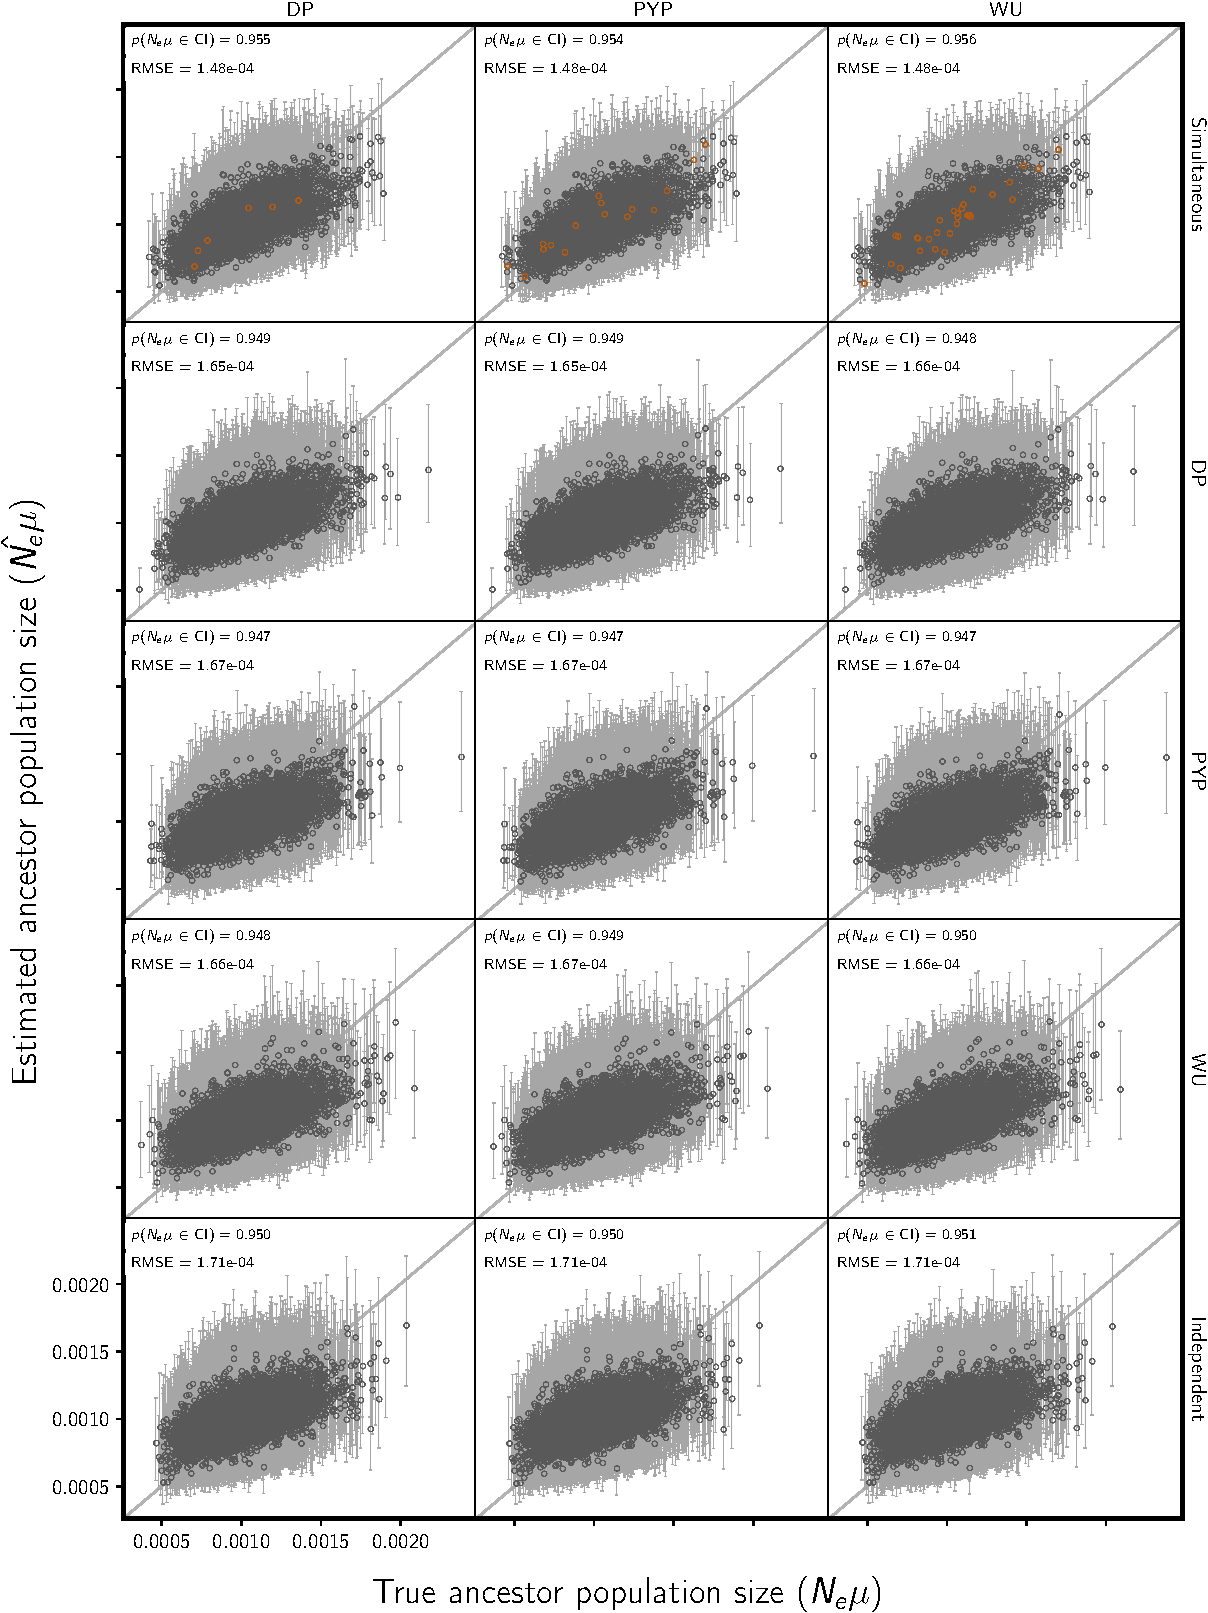
\includegraphics[width=\textwidth,height=0.9\textheight,keepaspectratio]{../images/from-project-repo/var-only-infer-columns-by-data-rows-ancestor-size-scatter-cropped.pdf}
        \captionsetup{name=Figure S, labelformat=noSpace, listformat=sFigList}
        \caption{\footnotesize
        The DP (left column),
        PYP (middle column),
        and
        \wunif
        perform similarly at estimating the effective size of the ancestral
        populations from only the variable characters from \datasets simulated
        under five different models (see row labels) with 10 pairs of
        populations.
        At the top of each plot is the root-mean-square error (RMSE)
        and
        the proportion of \datasets for which the true population size was
        included in the 95\% credible interval---$p(\epopsize\murate \in
        \textrm{CS})$.
        Estimates for which the potential-scale reduction factor was greater
        than 1.2 \citep{Brooks1998} are highlighted in orange.
        We generated the plot using matplotlib Version 3.1.3
        \citep{matplotlib}.
        }
        \label{fig:varonlyancpopsizegrid}
    \end{center}
\end{figure}

\begin{figure}[htbp]
    \begin{center}
        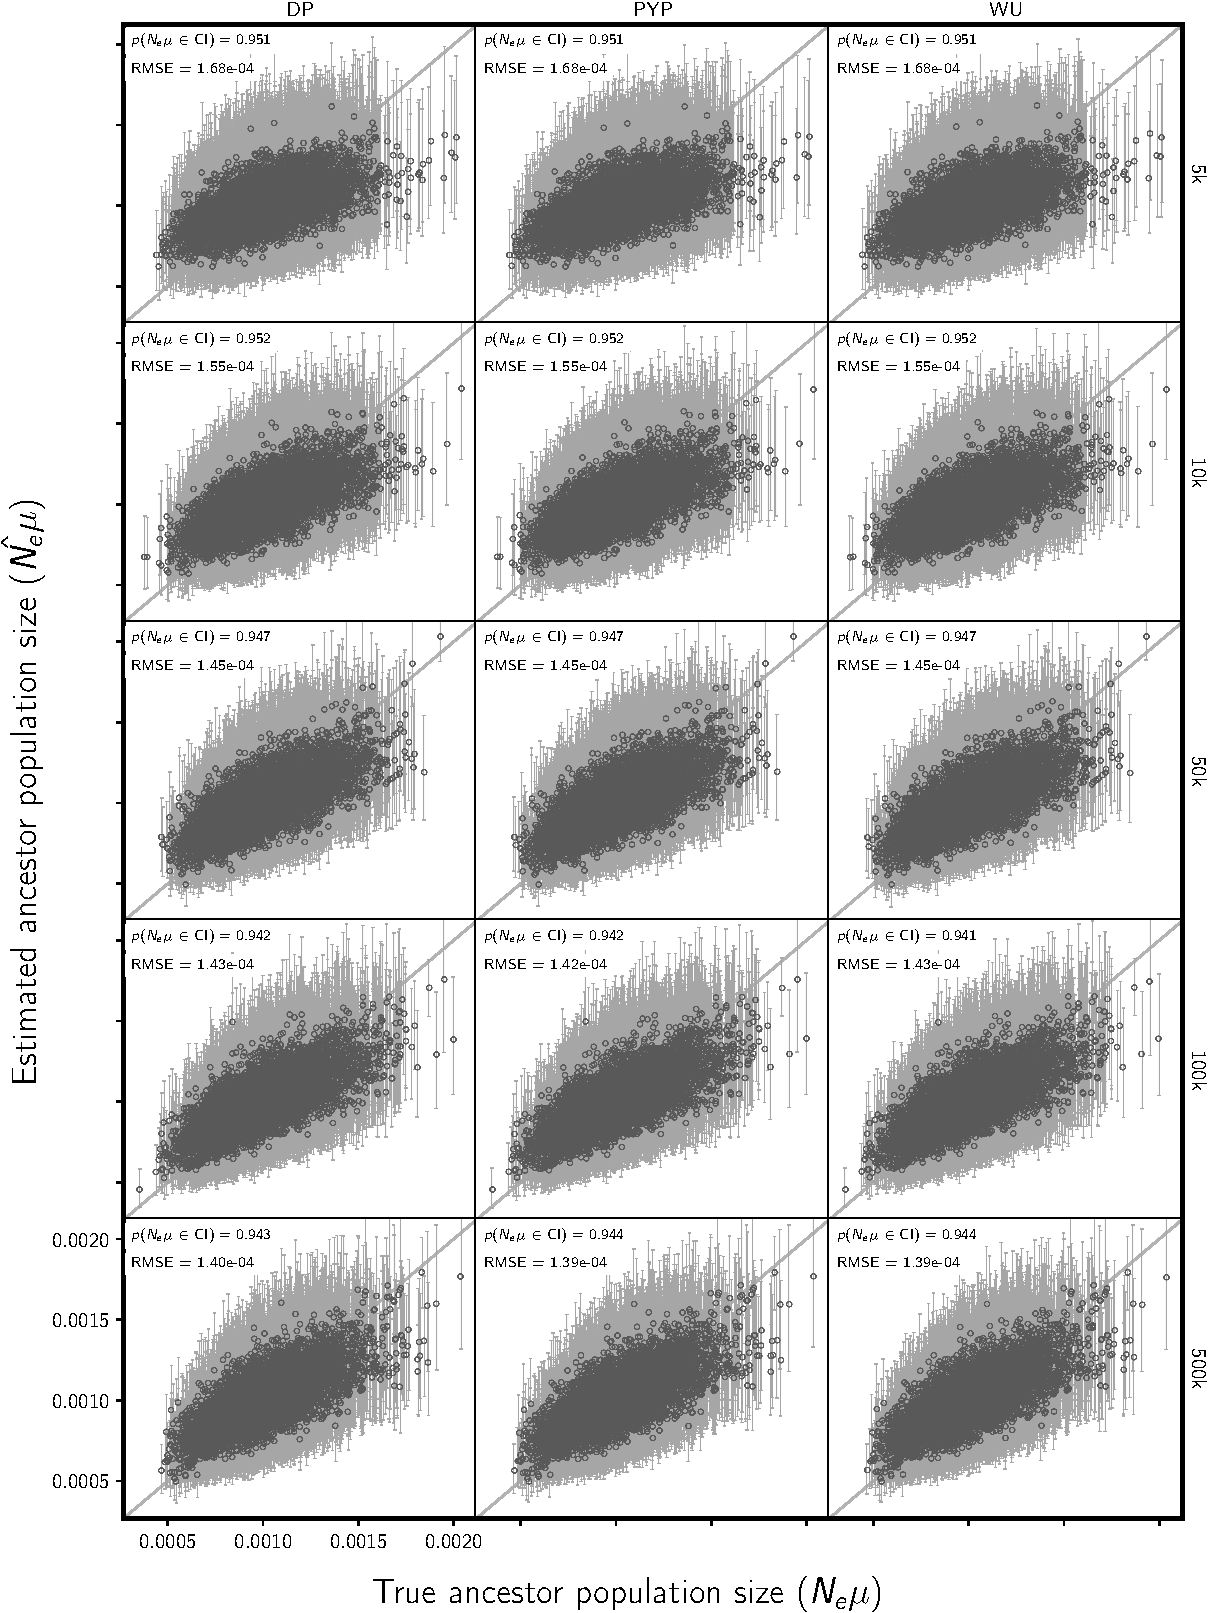
\includegraphics[width=\textwidth,height=0.9\textheight,keepaspectratio]{../images/from-project-repo/nchars-ancestor-size-scatter-cropped.pdf}
        \captionsetup{name=Figure S, labelformat=noSpace, listformat=sFigList}
        \caption{\footnotesize
        The DP (left column),
        PYP (middle column),
        and
        \wunif
        perform similarly well at estimating the effective size of the
        ancestral populations from \datasets of varying size (see row labels)
        simulated with 10 pairs of populations diverging independently.
        At the top of each plot is the root-mean-square error (RMSE)
        and
        the proportion of \datasets for which the true population size was
        included in the 95\% credible interval---$p(\epopsize\murate \in
        \textrm{CS})$.
        Estimates for which the potential-scale reduction factor was greater
        than 1.2 \citep{Brooks1998} are highlighted in orange.
        We generated the plot using matplotlib Version 3.1.3
        \citep{matplotlib}.
        }
        \label{fig:ancpopsizegridbysize}
    \end{center}
\end{figure}

\begin{figure}[htbp]
    \begin{center}
        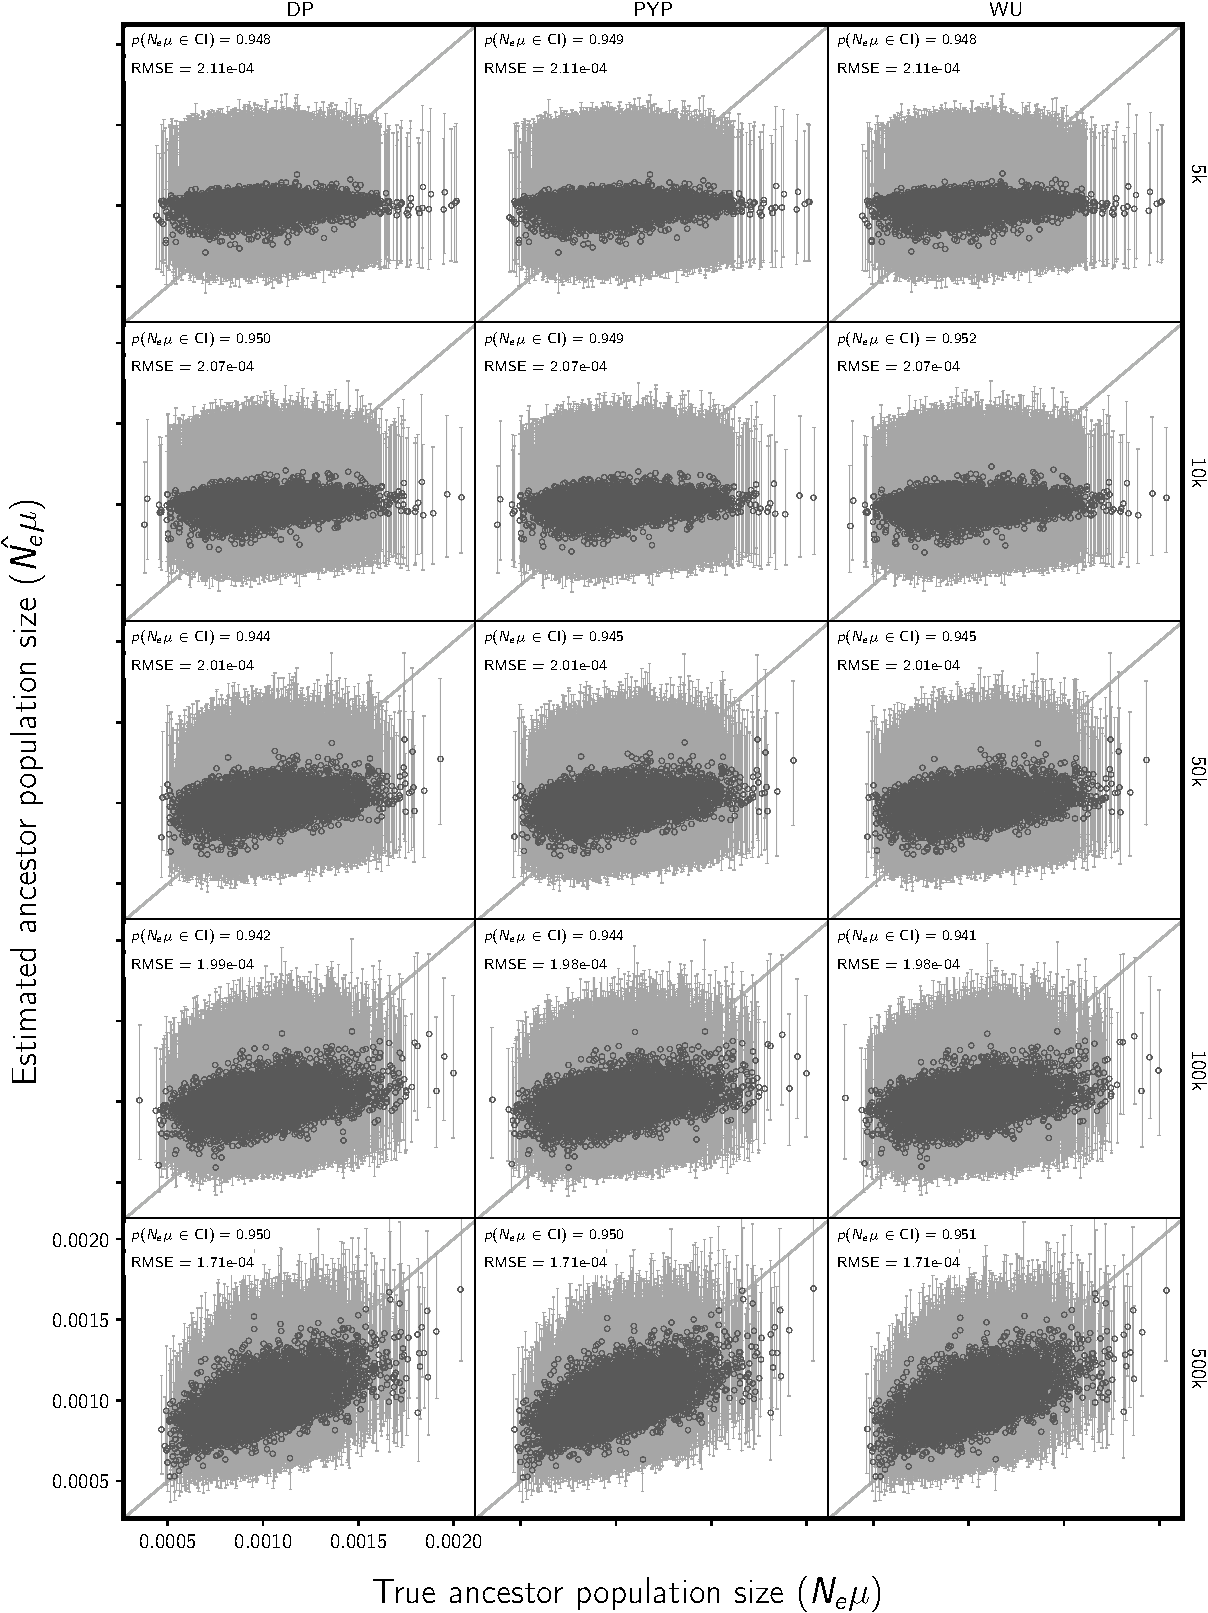
\includegraphics[width=\textwidth,height=0.9\textheight,keepaspectratio]{../images/from-project-repo/var-only-nchars-ancestor-size-scatter-cropped.pdf}
        \captionsetup{name=Figure S, labelformat=noSpace, listformat=sFigList}
        \caption{\footnotesize
        The DP (left column),
        PYP (middle column),
        and
        \wunif
        perform similarly at estimating the effective size of the ancestral
        populations from only the variable characters from \datasets of varying
        size (see row labels) simulated with 10 pairs of populations diverging
        independently.
        At the top of each plot is the root-mean-square error (RMSE)
        and
        the proportion of \datasets for which the true population size was
        included in the 95\% credible interval---$p(\epopsize\murate \in
        \textrm{CS})$.
        Estimates for which the potential-scale reduction factor was greater
        than 1.2 \citep{Brooks1998} are highlighted in orange.
        We generated the plot using matplotlib Version 3.1.3
        \citep{matplotlib}.
        }
        \label{fig:varonlyancpopsizegridbysize}
    \end{center}
\end{figure}


% Descendant population size

\begin{figure}[htbp]
    \begin{center}
        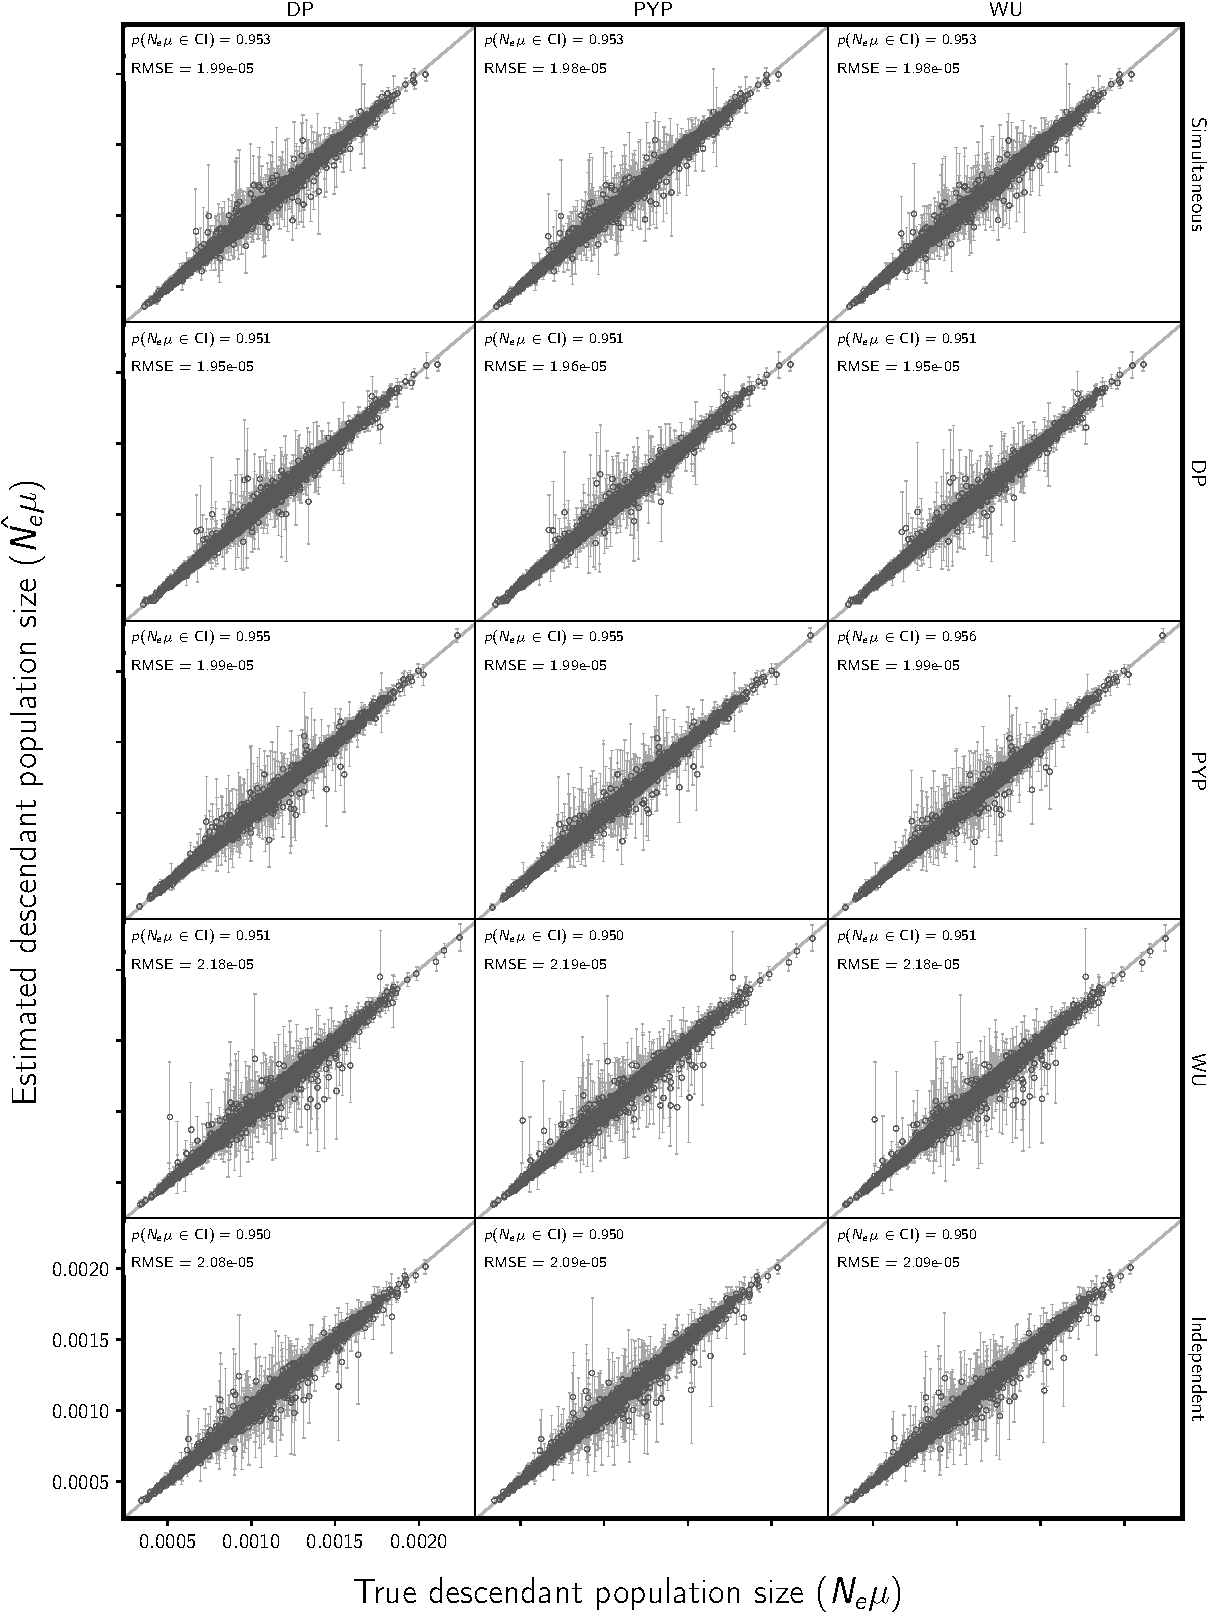
\includegraphics[width=\textwidth,height=0.9\textheight,keepaspectratio]{../images/from-project-repo/infer-columns-by-data-rows-descendant-size-scatter-cropped.pdf}
        \captionsetup{name=Figure S, labelformat=noSpace, listformat=sFigList}
        \caption{\footnotesize
        The DP (left column),
        PYP (middle column),
        and
        \wunif
        perform similarly at estimating the effective size of the
        descendant populations from \datasets simulated under five different
        models (see row labels) with 500,000 characters from 10 pairs of
        populations.
        At the top of each plot is the root-mean-square error (RMSE)
        and
        the proportion of \datasets for which the true population size was
        included in the 95\% credible interval---$p(\epopsize\murate \in
        \textrm{CS})$.
        Estimates for which the potential-scale reduction factor was greater
        than 1.2 \citep{Brooks1998} are highlighted in orange.
        We generated the plot using matplotlib Version 3.1.3
        \citep{matplotlib}.
        }
        \label{fig:descpopsizegrid}
    \end{center}
\end{figure}

\begin{figure}[htbp]
    \begin{center}
        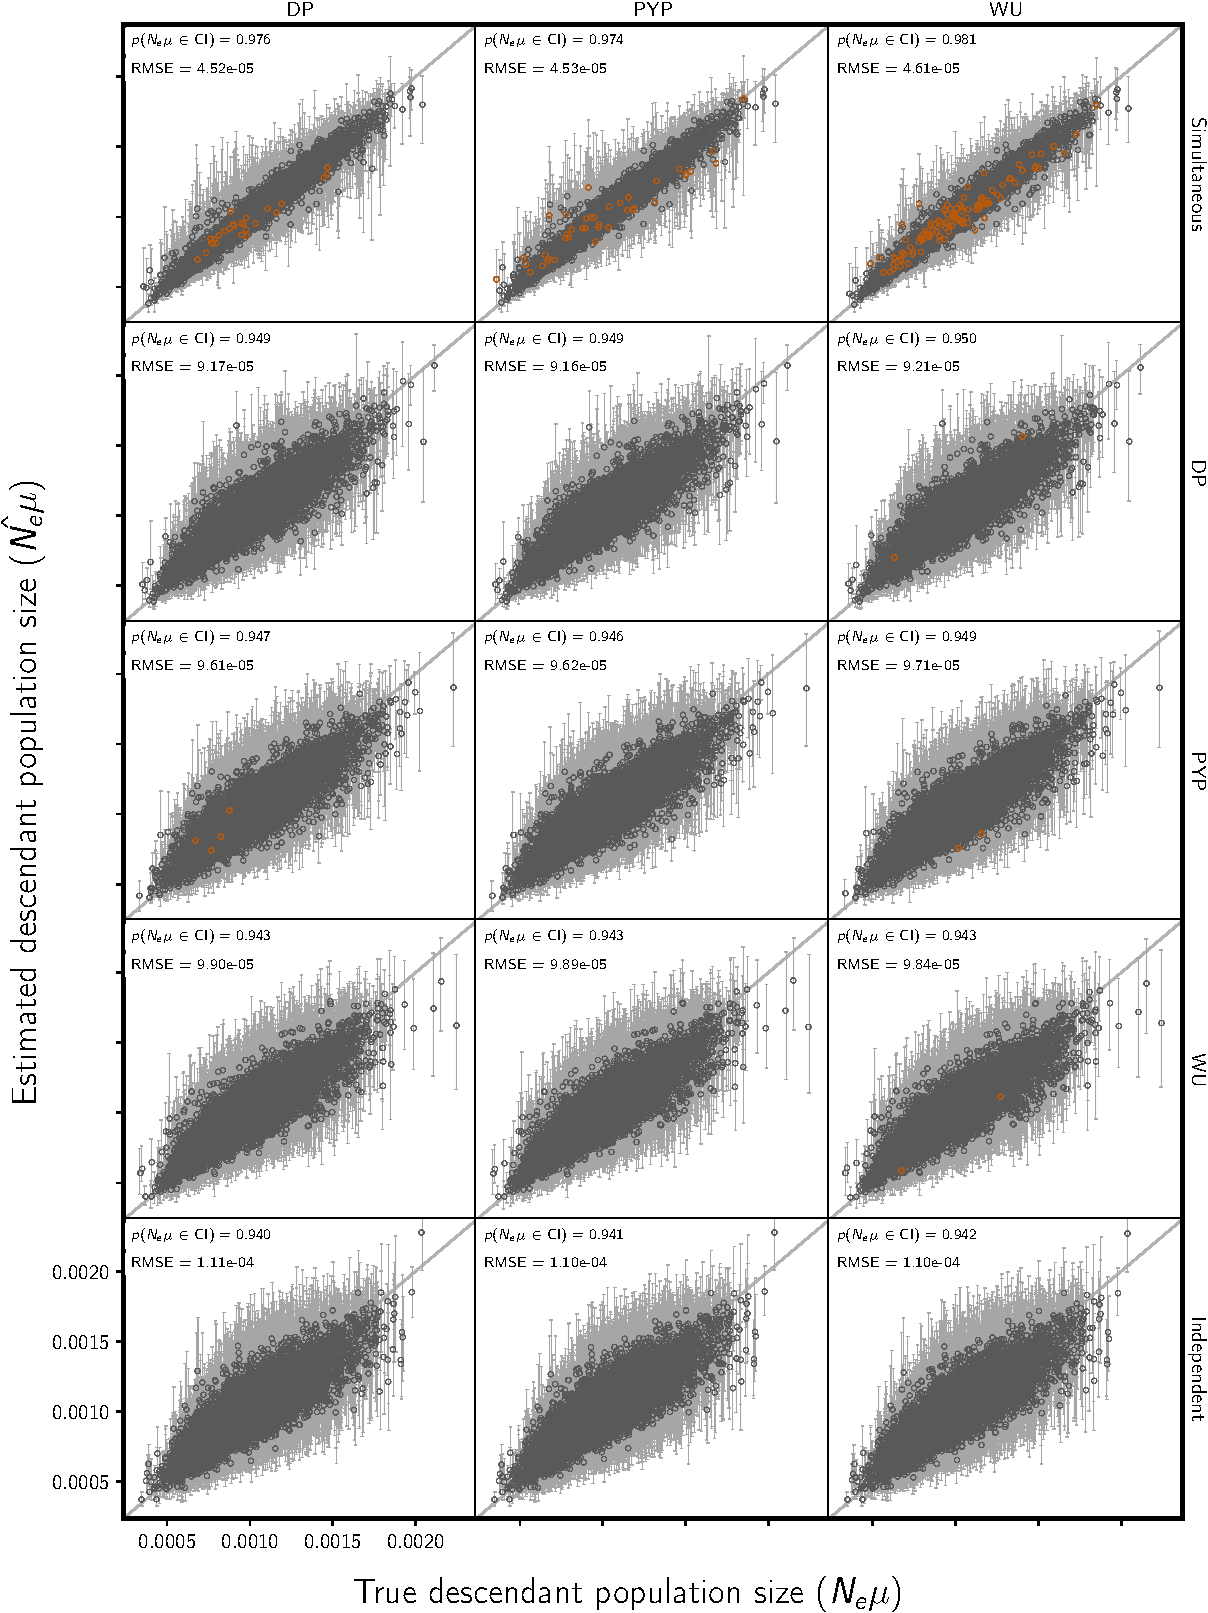
\includegraphics[width=\textwidth,height=0.9\textheight,keepaspectratio]{../images/from-project-repo/var-only-infer-columns-by-data-rows-descendant-size-scatter-cropped.pdf}
        \captionsetup{name=Figure S, labelformat=noSpace, listformat=sFigList}
        \caption{\footnotesize
        The DP (left column),
        PYP (middle column),
        and
        \wunif
        perform similarly at estimating the effective size of the descendant
        populations from only the variable characters from \datasets simulated
        under five different models (see row labels) with 10 pairs of
        populations.
        At the top of each plot is the root-mean-square error (RMSE)
        and
        the proportion of \datasets for which the true population size was
        included in the 95\% credible interval---$p(\epopsize\murate \in
        \textrm{CS})$.
        Estimates for which the potential-scale reduction factor was greater
        than 1.2 \citep{Brooks1998} are highlighted in orange.
        We generated the plot using matplotlib Version 3.1.3
        \citep{matplotlib}.
        }
        \label{fig:varonlydescpopsizegrid}
    \end{center}
\end{figure}

\begin{figure}[htbp]
    \begin{center}
        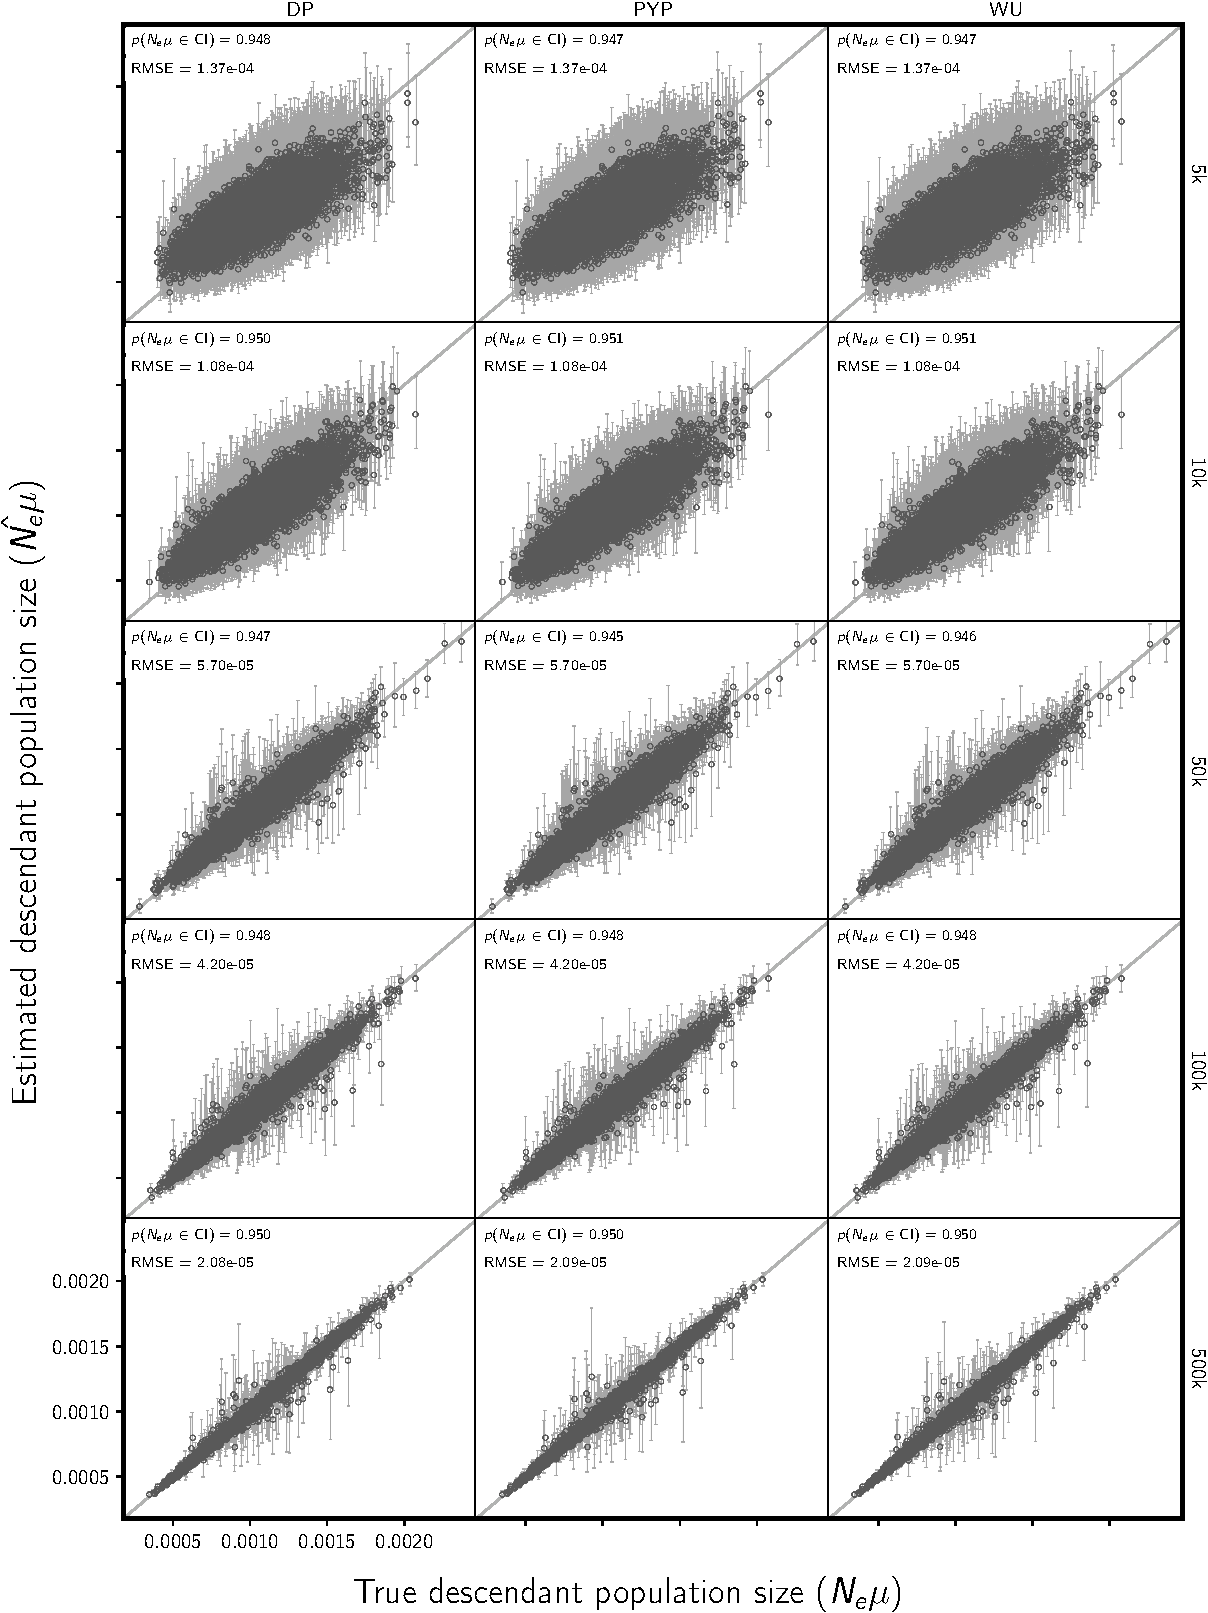
\includegraphics[width=\textwidth,height=0.9\textheight,keepaspectratio]{../images/from-project-repo/nchars-descendant-size-scatter-cropped.pdf}
        \captionsetup{name=Figure S, labelformat=noSpace, listformat=sFigList}
        \caption{\footnotesize
        The DP (left column),
        PYP (middle column),
        and
        \wunif
        perform similarly well at estimating the effective size of the
        descendant populations from \datasets of varying size (see row labels)
        simulated with 10 pairs of populations diverging independently.
        At the top of each plot is the root-mean-square error (RMSE)
        and
        the proportion of \datasets for which the true population size was
        included in the 95\% credible interval---$p(\epopsize\murate \in
        \textrm{CS})$.
        Estimates for which the potential-scale reduction factor was greater
        than 1.2 \citep{Brooks1998} are highlighted in orange.
        We generated the plot using matplotlib Version 3.1.3
        \citep{matplotlib}.
        }
        \label{fig:descpopsizegridbysize}
    \end{center}
\end{figure}

\begin{figure}[htbp]
    \begin{center}
        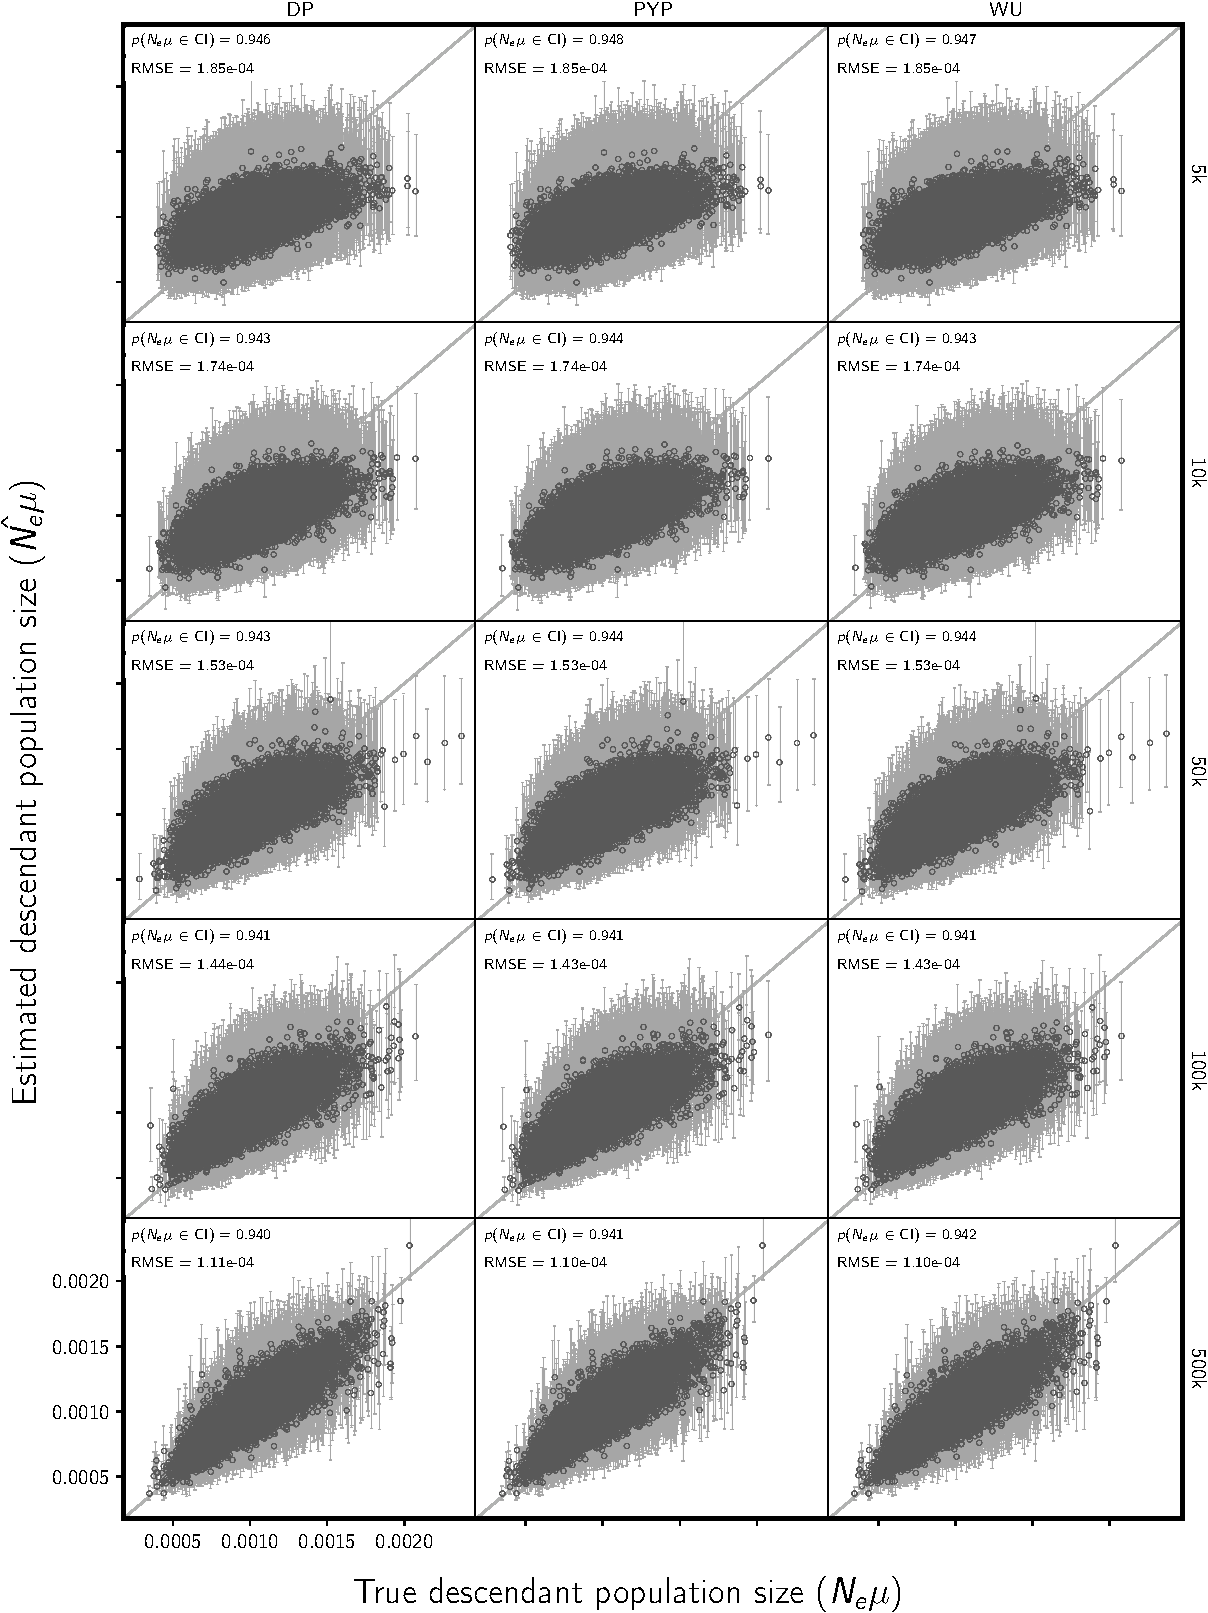
\includegraphics[width=\textwidth,height=0.9\textheight,keepaspectratio]{../images/from-project-repo/var-only-nchars-descendant-size-scatter-cropped.pdf}
        \captionsetup{name=Figure S, labelformat=noSpace, listformat=sFigList}
        \caption{\footnotesize
        The DP (left column),
        PYP (middle column),
        and
        \wunif
        perform similarly at estimating the effective size of the descendant
        populations from only the variable characters from \datasets of varying
        size (see row labels) simulated with 10 pairs of populations diverging
        independently.
        At the top of each plot is the root-mean-square error (RMSE)
        and
        the proportion of \datasets for which the true population size was
        included in the 95\% credible interval---$p(\epopsize\murate \in
        \textrm{CS})$.
        Estimates for which the potential-scale reduction factor was greater
        than 1.2 \citep{Brooks1998} are highlighted in orange.
        We generated the plot using matplotlib Version 3.1.3
        \citep{matplotlib}.
        }
        \label{fig:varonlydescpopsizegridbysize}
    \end{center}
\end{figure}
